% Preamble
    \documentclass[12pt]{article}

    % Margin control
        \usepackage[margin=.75in]{geometry}
        \usepackage{array}

        \newenvironment{amatrix}[1]{%
            \left[\begin{array}{@{}*{#1}{c}|c@{}}
        }{%
            \end{array}\right]
        }

    % Better enumerate control
        \usepackage{enumerate}
        \usepackage{enumitem}

    % Standard
        \usepackage{amssymb}
        \usepackage{amsthm}
        \usepackage{amsmath}

    % Pictures
        \usepackage{graphicx}
        \graphicspath{ {images/} }

    % Header/Footer
        \usepackage{fancyhdr}
        \setlength{\headheight}{15pt}
        \pagestyle{fancy}
        \lhead{Chad Collins}
        \chead{Math 459 Portfolio}
        \rhead{\today}
        \cfoot{}
        \rfoot{\thepage}

    % Columns
        \usepackage{multicol}

    % Diagrams
        \usepackage{tikz-cd}
        \usepackage{mathtools}

    % No indent
        \setlength\parindent{0pt}
        \setlength{\parskip}{1em}

    % Convenient mappings
        \newcommand{\N}{\mathbb{N}}
        \newcommand{\Z}{\mathbb{Z}}
        \newcommand{\Q}{\mathbb{Q}}
        \newcommand{\C}{\mathbb{C}}
        \newcommand{\R}{\mathbb{R}}
        \newcommand{\RP}{\mathbb{RP}}
        \newcommand{\PP}{\mathbb{P}}
        \newcommand{\contradiction}{\Rightarrow \Leftarrow}
        \let\ds\displaystyle

    % Exercise environment
        \newenvironment{exercise}[2][Exercise]{\begin{trivlist}
        \item[\hskip \labelsep {\bfseries #1}\hskip \labelsep {\bfseries #2.}]}{\end{trivlist}}

        \newenvironment{theorem}[2][Theorem]{\begin{trivlist}
        \item[\hskip \labelsep {\bfseries #1}\hskip \labelsep {\bfseries #2.}]}{\end{trivlist}}
    % Solution environment
        \newenvironment{solution}
        {\begin{proof}[Solution]}
                    {\end{proof}}

\begin{document}
\begin{exercise}{1}
    Is it possible to construct a regular lattice 3-gon (i.e. an equilateral and equiangular lattice triangle)? If so, provide an example. If not, prove it.
    \begin{solution}
        It is not possible to construct a regular lattice 3-gon.

        Suppose not, that there exists a regular lattice 3-gon. Without loss of generality, assume one vertex is the origin, \( ( 0,0 ) \) and that the others are \( (m,n) \) and \( (a,b) \) for some \( a,b,m,n \in \Z \). Since the triangle is equilateral, we know the distances between each of the points are equal. Applying the distance formula yields the equality:
        \begin{align*}
            a^2+b^2 = m^{2} + n^{2} = (a-m)^{2} + ( b-n )^{2}.
        \end{align*}
        Expanding and considering the right most equality,
        \begin{align*}
            m^{2} + n^{2} &= a^{2} - 2am + m^{2} + b^{2} - 2bn + n^{2}\\
            a^{2} + b^{2}  &= 2 ( am + bn )\\
            \implies a^{2} + b^{2} &= m^{2} + n^{2} = 2(am + bn).
        \end{align*}
        We move to square, making use of the left most equality:
        \begin{align*}
            (a^{2} + b^{2} ) ( m^{2} + n^{2} ) &= 4 ( am + bn )^{2} \\
            a^{2} m^{2} + a^{2} n^{2} + b^{2} m^{2} + b^{2}n^{2} &= 4 a^{2} m^{2} + 8ambn + 4b^{2} n^{2} \\
            a^{2} n^{2} - 2ambn + b^{2} m^{2} &= 3(a^{2} m^{2} + 2ambn + b^{2} n^{2} ) \\
            (an-bm)^{2} &= 3(am+bn)^{2}.
        \end{align*}
        The last equality is impossible, since the calculation happens in \( \Z. \) Since \( (an-bm)^{2}  \) is a perfect square, \( 3 ( am+bn )^{2} \) must also be a perfect square, but 3 is not a perfect square. In other words, \( \left| an-bm \right| = \left| \sqrt{3} (am+bn) \right| \notin \Z \).
    \end{solution}
\end{exercise}

\begin{exercise}{2}
    Is it possible to construct a regular lattice 4-gon (i.e. a square)? If so, provide an example. If not, prove it.
    \begin{solution}
        See the figure below.
        \begin{center}
        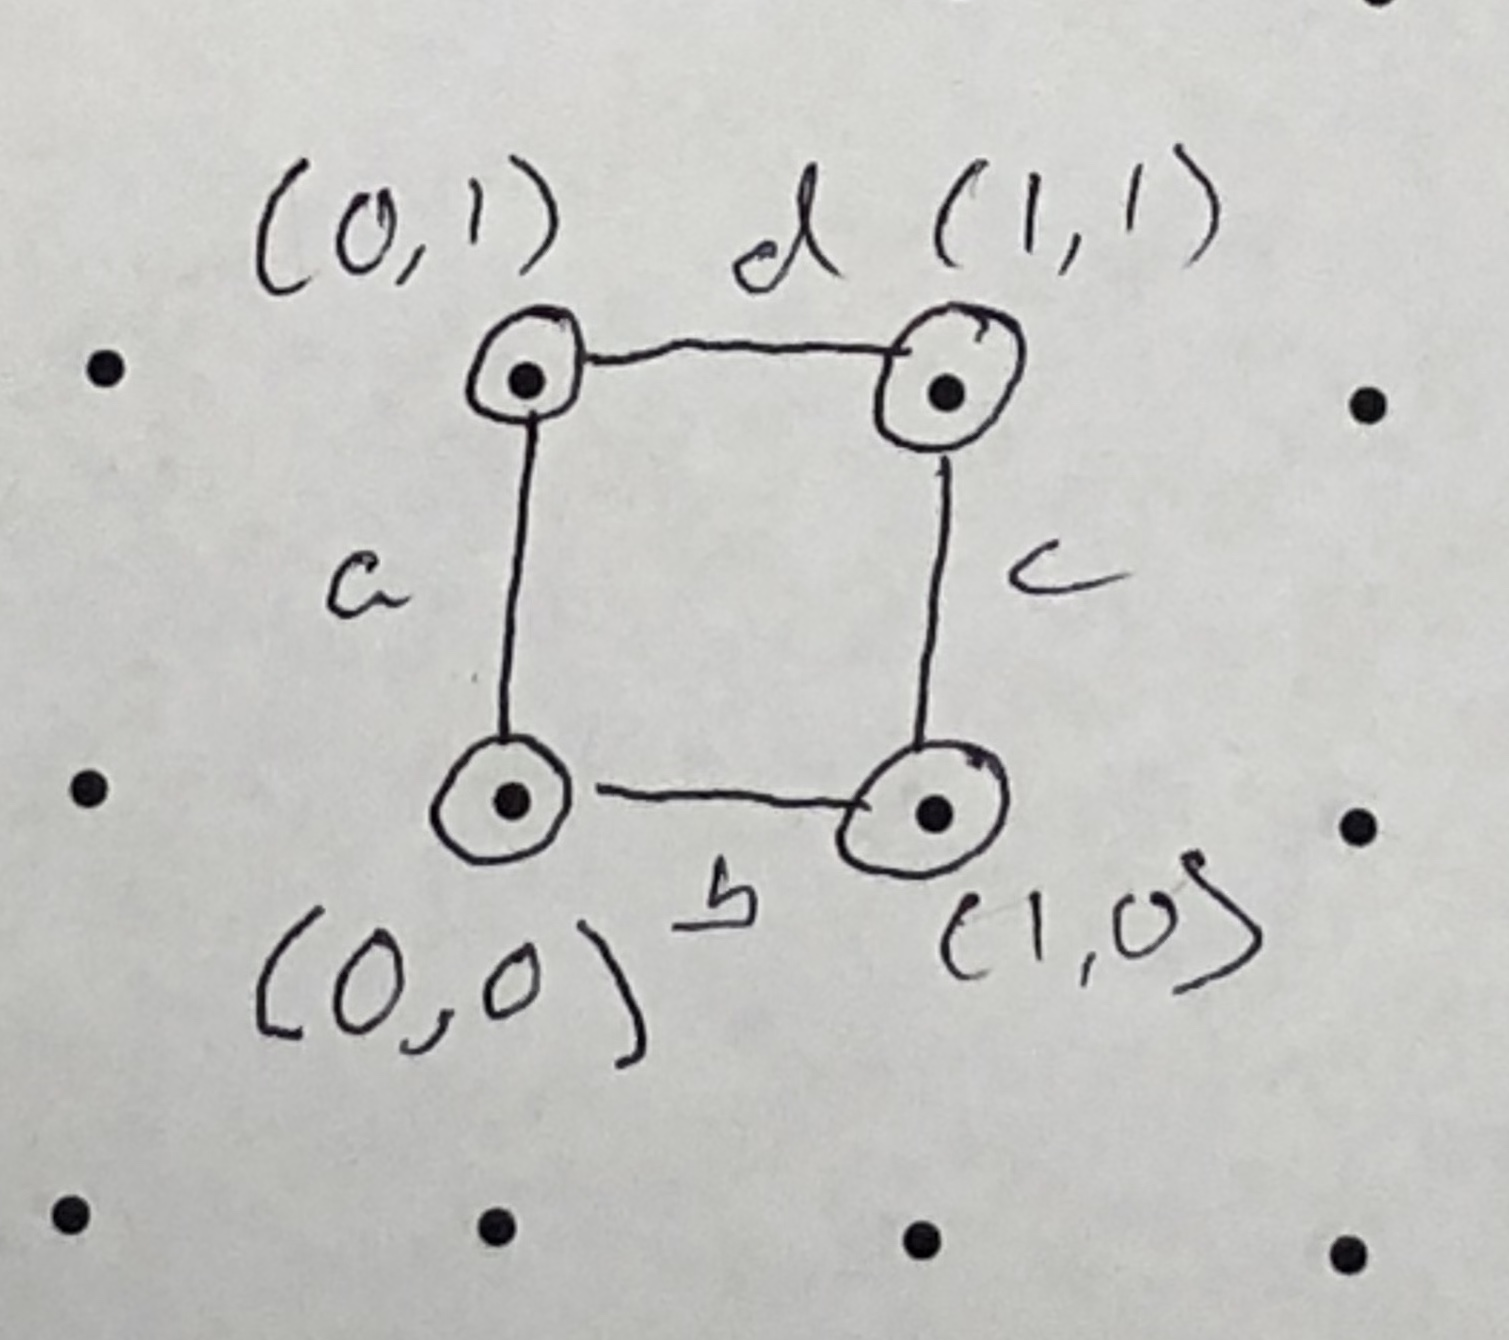
\includegraphics[width=.3\linewidth]{2}
        \end{center}
        Here, \( a = \sqrt{0^{2} + 1^{2}} = 1, \ b = \sqrt{1^{2} + 0^{2}} = 1, \ c = \sqrt{(1-1)^{2} + 1^{2}} = 1, \) and \( d = \sqrt{1^{2} + ( 1-1 )^{2}} =1 \). Thus \( a=b=c=d \). Moreover, the angles are congruent as well. By the definition of dot product, \( <1,0> \cdot <0,1> = \left| <1,0> \right| \left| <0,1> \right| \cos \theta \implies 0 = \cos \theta \implies \theta = \pi/2.\) Similar calculations reveal the other angles have the same measure.
    \end{solution}
\end{exercise}

\begin{exercise}{3}
    Is it possible to construct a regular lattice pentagon (5-gon)? If so, provide an example. If not, prove it.
    \begin{solution}
        Such a construction is not possible.

        Suppose not, that there exists a regular lattice pentagon. Without loss of generality, suppose one vertex of this figure is the origin, \( ( 0,0 ). \) Let \( (a,b) \) and \( ( m,n ) \) be two other lattice vertices on either side of the origin. Consider the vectors \( \langle a,b \rangle \) and \( \langle m,n \rangle . \) Since our polygon is regular, we know \( \left| \langle a,b \rangle \right| = \left| \langle m,n \rangle \right| .\) Moreover, we know that each interior angle of a regular pentagon has measure \( 3\pi/5. \) Armed with this knowledge, we compute the dot product between the two vectors,
        \begin{align*}
            \langle a,b \rangle \cdot \langle m,n \rangle &= \left|\langle a,b\rangle \right| \left|\langle m,n \rangle\right| \cos \frac{3\pi}{5}  \\
            am + bn &= \left| \langle a,b \rangle \right|^{2} \cos \frac{3\pi}{5} \\
            am + bn &= (a^{2} + b^{2} ) \cos \frac{3\pi}{5} \\
            \implies\cos \frac{3\pi}{5} &= \frac{am+bn}{a^{2} + b^{2}} .
        \end{align*}
        Note that the last move is legal since not both of \( a \) and \( b \) are 0, since \( \langle a,b \rangle \) is the side of a polygon. We claim that \( \cos 3\pi/5 \) is irrational, making the last equality impossible since the right hand side is rational. We have a contradiction, and thus there cannot exist a regular lattice pentagon.
    \end{solution}
\end{exercise}

\begin{exercise}{4}
    Show that the cosine of the interior and exterior angle of any regular lattice polygon must be rational. Hint: use vectors and the dot product.
    \begin{solution}
        We intend to generalize our approach from problem 3. Suppose we have a regular lattice polygon and that the cosine of the interior angle of the polygon is irrational. We can identify three adjacent vertices to create two vectors \( u \) and \( v. \) Since the polygon is regular, \( \left| u \right| = \left| v \right| .  \) Suppose that \( u = \langle a,b \rangle \) and \( v = \langle c,d \rangle . \) We know that \( u \) and \( v \) consist of only integer parts since each vertex of the polygon is a lattice point, and thus each component is the difference of two integers. We compute the dot product between the two vectors, with \( \theta \) as the interior angle of the polygon.
        \begin{align*}
            u \cdot v &= \left| u \right| \left| v \right| \cos\theta\\
            ac + bd &= \left| \langle a,b \rangle  \right|^{2} \cos\theta\\
            ac + bd &= a^{2} + b^{2} \cos\theta\\
            \implies\frac{ac + bd}{a^{2} + b^{2}} &= \cos\theta.
        \end{align*}
        Note that the last move is legal since not both of \( a \) and \( b \) can be 0, since \( \langle a,b \rangle \) is the side of a polygon. We have a contradiction since we assumed that \( \cos\theta \) is irrational and we have shown that it is rational.

        For the cosine of the exterior angle, first recall the classic identity: \( \cos ( \pi - \theta ) = -\cos\theta \). Notice that the exterior angle of a polygon is simply the supplement of the interior. Thus if \( \theta \) is the interior angle of our polygon, \( \pi-\theta \) is the exterior angle. Now, suppose we had a regular lattice polygon where the cosine of the exterior angle of said polygon is irrational. We can express this angle as \( \pi-\theta \) where \( \theta \) is the interior angle, so \( \cos(\pi-\theta)=-\cos\theta \notin \Q \) by assumption. If \( -\cos\theta\notin\Q \), then \( \cos\theta\notin\Q. \) We showed in the first part of the problem that the cosine of the interior angle of a regular lattice polygon must be rational, so we have a contradiction.
    \end{solution}
\end{exercise}

\begin{exercise}{5}
    Use exercise 4 to show that it is not possible to construct a regular lattice octagon (8-gon).
    \begin{solution}
        Recall that the measure of the interior angles of a regular 8-gon is \( 3\pi/4. \) Now \( \cos 3\pi/4 = \sqrt{3} /2 \notin \Q.\) By exercise 4, it is not possible to construct a regular lattice octagon.
    \end{solution}
\end{exercise}

\begin{exercise}{6}
    Show that if \(\alpha\) is a lattice angle and if the measure of \(\alpha\) is not equal to \( \pi/2 \) or an odd integer multiple of \( \pi/2 \), then the tangent of \(\alpha\) is a rational number.
    \begin{solution}
        Any lattice angle will lie between two lattice lines, and thus we can construct vectors on the lattice lines whose endpoints are lattice points. Let the vectors which lie on either side of \( \alpha \) be \( \langle a,b \rangle \) and \( \langle c,d \rangle \) where \( a,b,c,d \in \Z. \) Note that every vector on the lattice plane will be of this form since both components are formed by subtraction of integers. Since we are interested in the tangent of \( \alpha \), we will consider first the cosine and sine of \( \alpha. \) To compute \( \cos\alpha, \) we compute the dot product between the two vectors,
        \begin{align*}
            \langle a,b \rangle \cdot \langle c,d \rangle &= \left| \langle a,b \rangle \right| \left| \langle c,d \rangle \right| \cos\alpha\\
            \implies\cos\alpha &= \frac{ac+bd}{\left| \langle a,b \rangle \right| \left| \langle c,d \rangle \right|}.
        \end{align*}
        Note that the last division is legal since both vectors are nonzero and thus have positive length. To compute \( \sin\alpha, \) we will compute a cross product between the two angles. To do this, we must project into \( \Z^{3} \) by simply adding a third 0 component to each vector.
        \begin{align*}
            \langle a,b,0 \rangle \times \langle c,d,0 \rangle =
            \begin{vmatrix}
                i & j & k\\
                a & b & 0\\
                c & d & 0
            \end{vmatrix} = k\begin{vmatrix}
                a & b\\
                c & d
            \end{vmatrix}= \langle 0,0,ab-cd \rangle.
        \end{align*}
        Note that \( \left| \langle a,b,0 \rangle \right| = \left| \langle a,b \rangle \right| \) and \( \left| \langle c,d,0 \rangle \right| = \left| \langle c,d \rangle \right| . \) Now we utilize the definition of the cross product:
        \begin{align*}
            \left| \langle a,b,0 \rangle \times \langle c,d,0 \rangle \right| &= \left| \langle a,b,0 \rangle \right| \left| \langle c,d,0 \rangle \right| \sin\alpha\\
            ab-cd &= \left| \langle a,b \rangle \right| \left| \langle c,d \rangle \right|\sin\alpha\\
            \implies \sin\alpha &= \frac{ab-cd}{\left| \langle a,b \rangle \right| \left| \langle c,d \rangle \right|}.
        \end{align*}\pagebreak

        Since \( \tan\alpha = \sin\alpha/\cos\alpha, \) we divide the two previous equalities for \( \sin\alpha \) and \( \cos\alpha \) to find tangent.
        \begin{align*}
            \tan\alpha &= \frac{\sin\alpha}{\cos\alpha}\\
            &= \frac{\displaystyle\frac{ab-cd}{\left| \langle a,b \rangle \right| \left| \langle c,d \rangle \right|}}{\displaystyle\frac{ac+bd}{\left| \langle a,b \rangle \right| \left| \langle c,d \rangle \right|}}\\
            &= \frac{ab-cd}{ac+bd}.
        \end{align*}
        Note that \( ac+bd\neq0 \) since \( ac+bd = \langle a,b \rangle \cdot \langle c,d \rangle = \left| \langle a,b \rangle \right| \left| \langle c,d \rangle \right| \cos\alpha\) and \( \cos\alpha \) is nonzero since \( \alpha \neq n\pi/4 \) for odd \( n \). Now \( \tan\alpha = \frac{ab-cd}{ac+bd} \in \Q \) since \( ab-cd \in \Z \) and \( ac+bd \in \Z. \)
    \end{solution}
\end{exercise}

\begin{exercise}{7}
    Make a conjecture about the positive integers \( n \) for which it is possible to construct a regular \( n \)-gon. Although you do not need to provide a formal proof of your conjecture here, you should provide sufficient justification and reasoning (beyond simply citing the exercises you have already solved above) to indicate why you believe your conjecture is valid.
    \begin{solution}
        We make the audacious conjecture that the only possible regular lattice \( n \)-gons are squares, i.e. \( n \) must be four. Any regular polygon must adhere to the strict constrictions set by previous problems, namely numbers 4 and 6. We need the cosine of the interior angle to be rational, and we also need the tangent of that angle to be rational (necessary to be a lattice angle). Since tangent is the quotient of sine and cosine, sine is forced to be rational as well. On the unit circle, this only occurs at multiples of \( \pi, \) but of course these angles will not form polygons. Thus, the only constructible regular lattice polygons are squares, since we have constructed one! Moreover, squares avoid the tangent condition enforced by problem 6 since problem 6 excludes angles which are odd multiples of \( \pi/2 \), and squares have angles of measure \( \pi/2. \)
    \end{solution}
\end{exercise}

\begin{exercise}{8}
    Is it possible to construct a lattice square whose area is not a perfect square? If so, provide an example. If not, prove it.
    \begin{solution}
        Consider the square below.
        \begin{center}
        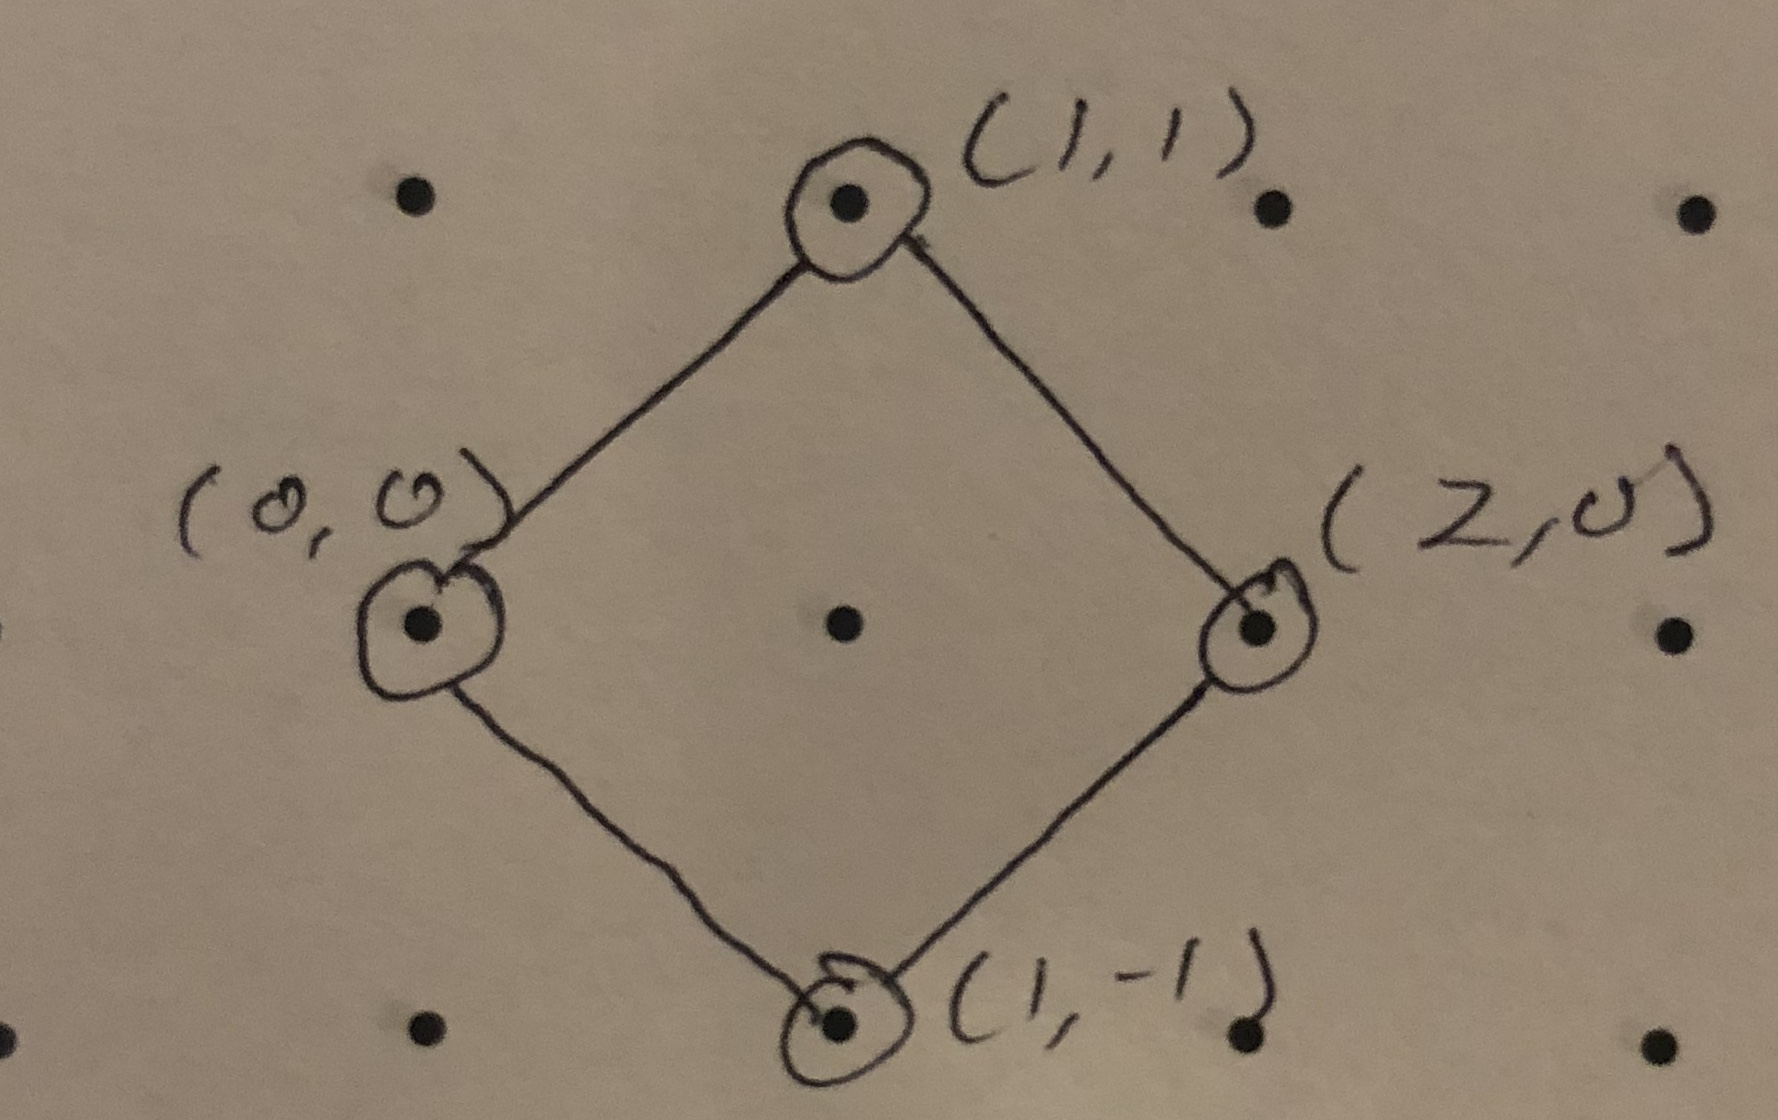
\includegraphics[width=.4\linewidth]{8}
        \end{center}
        Each side has length \( \sqrt{2} , \) and thus the square has area \( \sqrt{2}^{2} = 2 \) and 2 is not a perfect square.
    \end{solution}
\end{exercise}

\begin{exercise}{9}
    Is it possible to construct a lattice square whose area is not an integer? If so, provide an example. If not, prove it.
    \begin{solution}
        This is not possible. Without loss of generality, assume our square has a vertex at the origin, \( (0,0) \). Let \( ( a,b ) \) be a vertex of the square connected to the origin by a side of the square. Then the square has area \( ( \sqrt{a^{2} + b^{2}} )^{2} = a^{2} + b^{2} \in \Z.  \) Thus every lattice square will have integer area.
    \end{solution}
\end{exercise}

\begin{exercise}{10}
    Show that there exists a lattice square with area \( n  ,\) where \( n \) is a positive integer, if and only if there exist non-negative integers \( a \) and \( b \) such that
    \begin{align*}
        n = a^{2} + b^{2} .
    \end{align*}
    \begin{solution}
        Suppose that there exists a lattice square with area \( n\in \Z^{+} . \) Our square must have two lattice points connected by an edge of the square. Let these points be \( ( a,b ) \) and \( ( c,d ) . \) Then the area of the square is given by \( ( \sqrt{( a-c )^{2} + ( b-d )^{2}} )^{2} = ( a-c )^{2} + ( b-d )^{2}. \) Note that \( ( a-c )^{2} = ( c-a )^{2} \) and \( ( b-d )^{2} = ( d-b )^{2} . \) So, without loss of generality, suppose \( a>c \) and \( b>d, \) so that \( a-c \) and \( b-d \) are non-negative. Moreover, \( a-c \in \Z \) and \( b-d \in \Z. \) Thus \( n \) is the sum of the squares of two non-negative integers.

        Conversely, suppose for a positive integer \( n \) there exist non-negative integers \( a \) and \( b \) such that
        \begin{align*}
            n = a^{2} + b^{2} .
        \end{align*}
        Consider the figure below.
        \begin{center}
        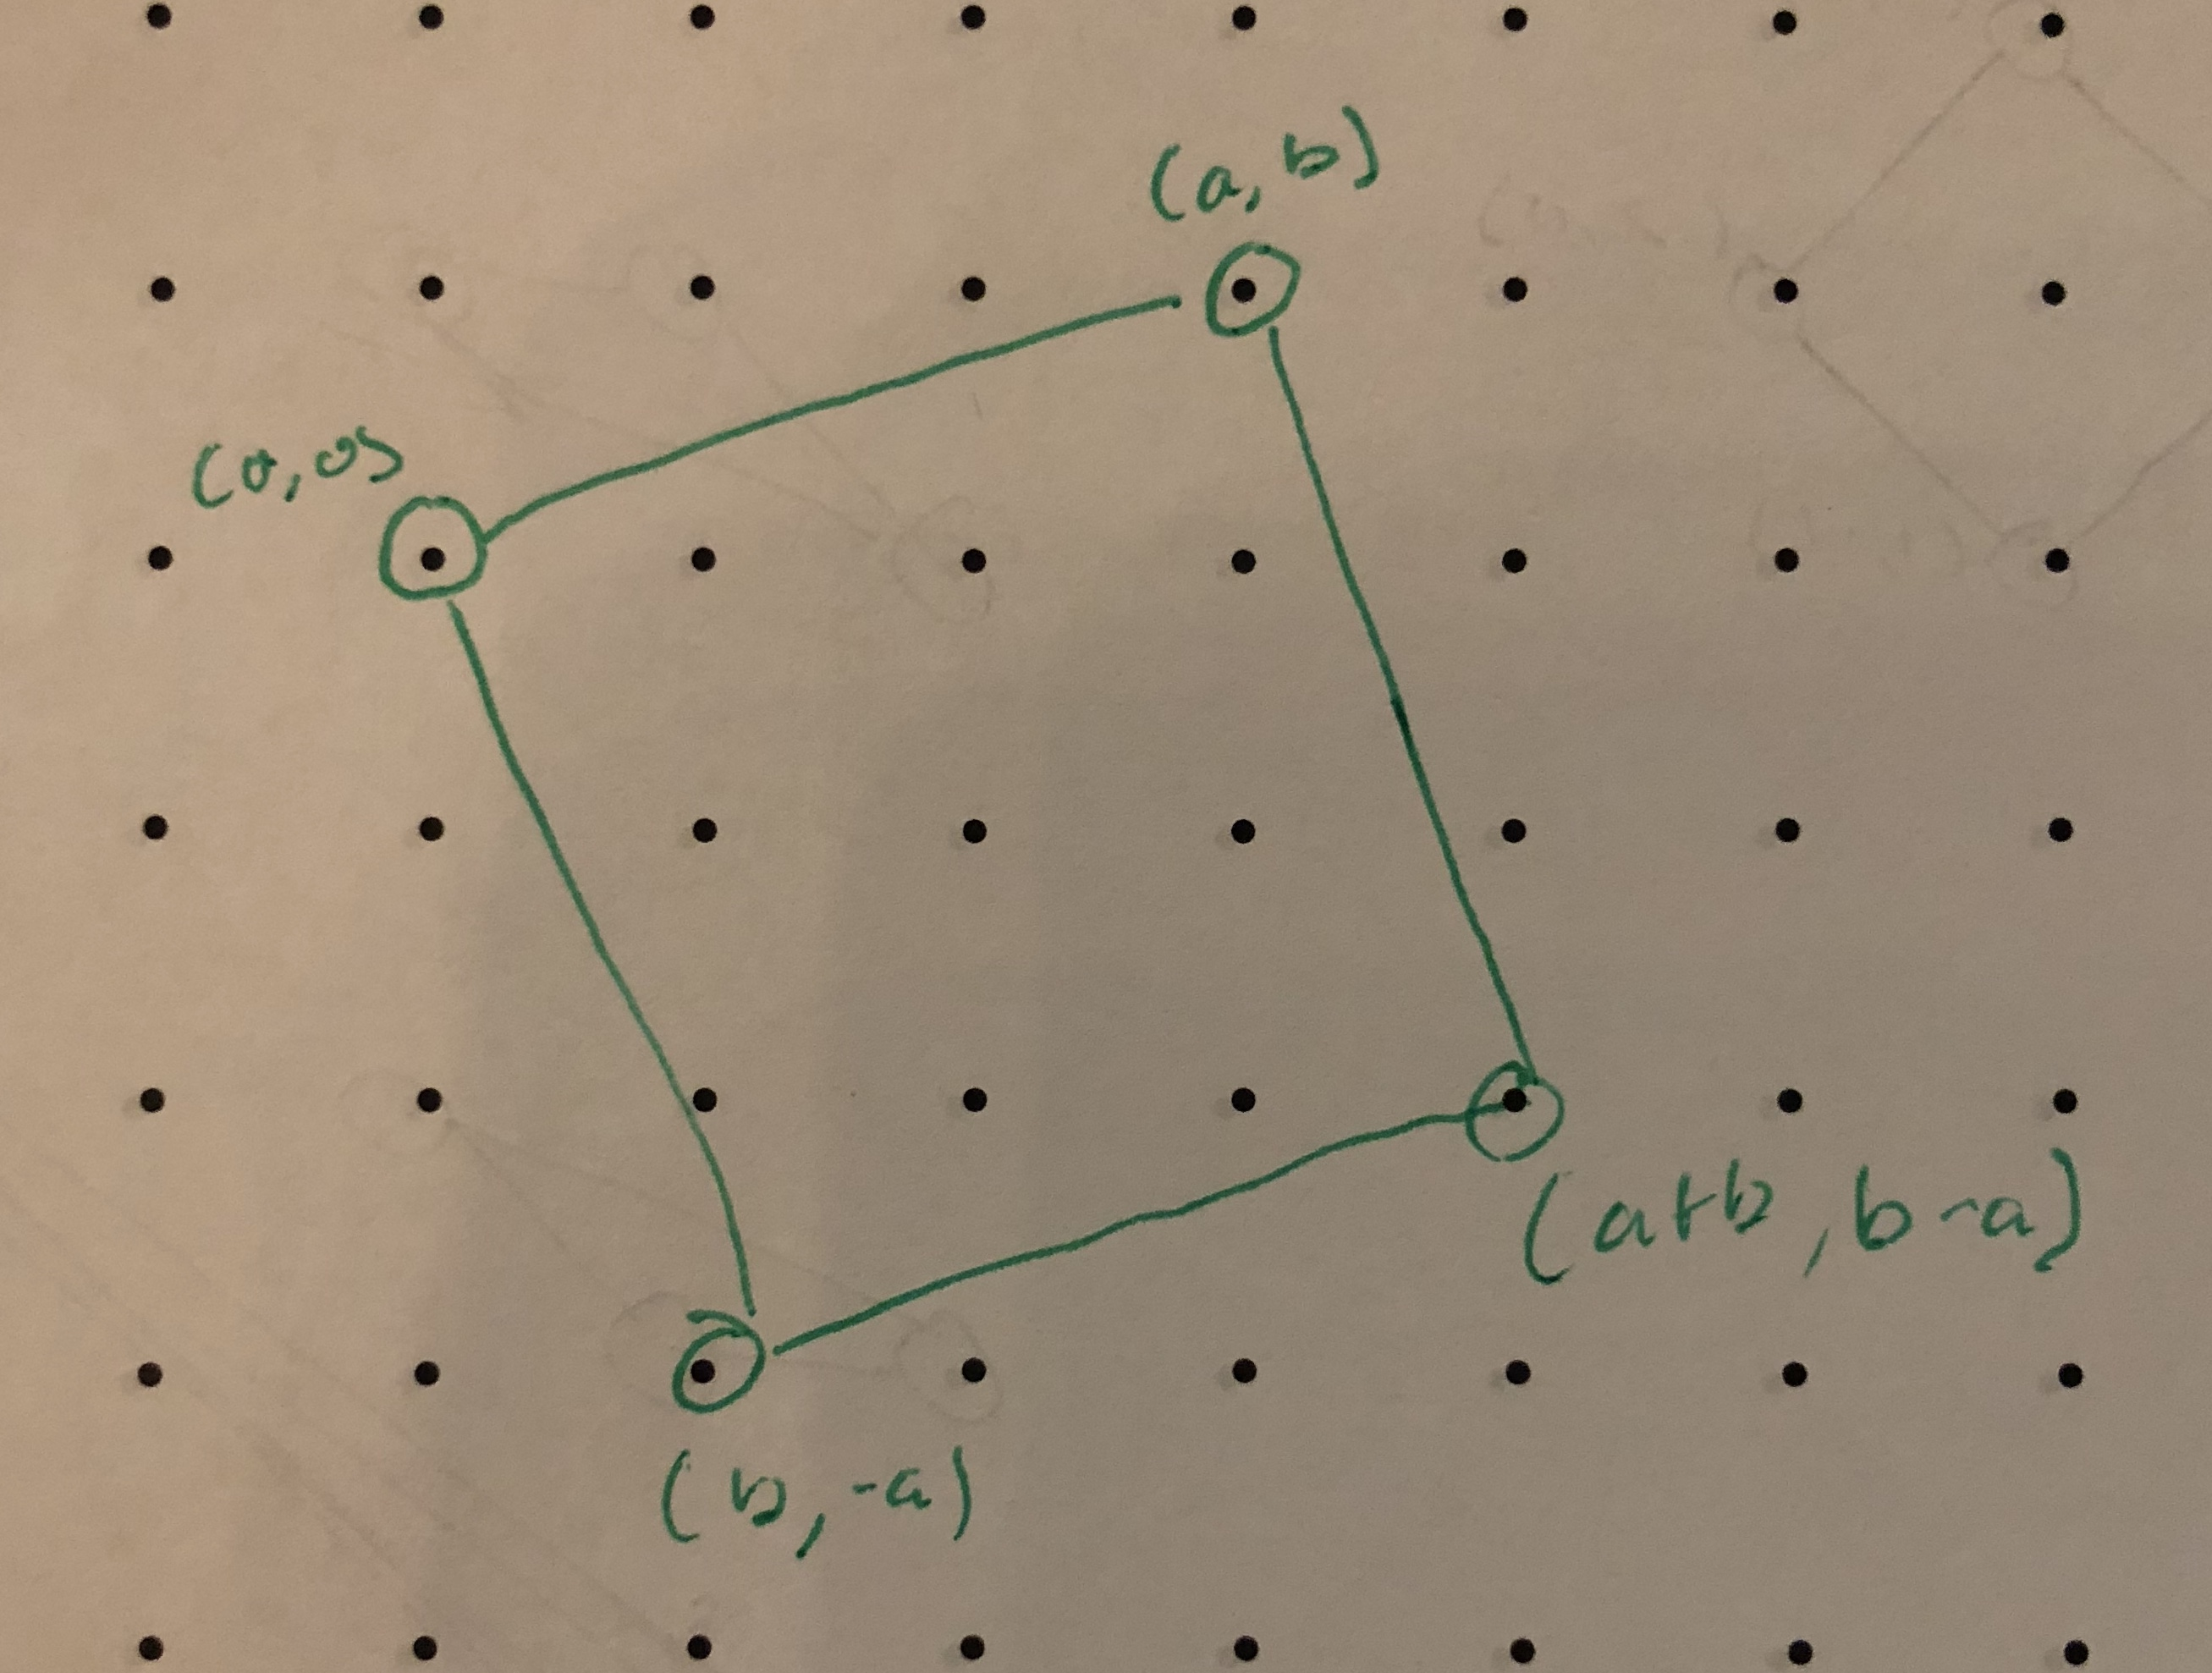
\includegraphics[width=.5\linewidth]{10}
        \end{center}
        Routine calculations will verify that each segment has length \( \sqrt{a^{2} + b^{2}} , \) and thus the area of the figure is \( a^{2} + b^{2} = n. \) Moreover, consider two of the vectors which make up the figure: \( \langle a,b \rangle \) and \( \langle b,-a \rangle . \) To compute the angle between the two vectors, we compute the dot product. Note that neither vector is the zero vector since \( n \neq 0. \)
        \begin{align*}
            \cos\theta &= \frac{\langle a,b \rangle \cdot \langle b,-a \rangle}{\left| \langle a,b \rangle \right| \left| \langle b,-a \rangle \right| } \\
            \cos\theta &= \frac{ab - ba}{\left| \langle a,b \rangle \right| \left| \langle b,-a \rangle \right| } \\
            \cos\theta &= 0 \text{ and so }\theta = \pi.
        \end{align*}
        Note that \( \theta \neq 3\pi/2 \) since the figure is convex. Similar calculations will verify that each angle has measure \( \pi. \) Thus the figure is a square with area \( n. \)
    \end{solution}
\end{exercise}

\begin{exercise}{11}
    Is it possible to construct a lattice triangle whose area is not an integer? If so, provide an example. If not, prove it.
    \begin{solution}
        Consider the triangle below.
        \begin{center}
        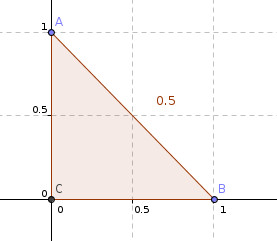
\includegraphics[width=.5\linewidth]{11}
        \end{center}
        This is indeed a lattice triangle with a base of length 1 and a height of length 1. Thus the area of the triangle is 1/2, which is decidedly not an integer.
    \end{solution}
\end{exercise}

\begin{exercise}{12}
    Construct (at least) 5 lattice polygons with different areas. Keep in mind that the polygons do not need to be convex! Find the area of each polygon. What do you observe? Make a conjecture about the possible values of the area of a lattice polygon based on your computation in this problem. For example, do you think it's possible to achieve all integer areas? All rational areas? All real areas?\pagebreak
    \begin{solution}
        The polygons are shown below, along with their areas.
        
        \begin{center}
        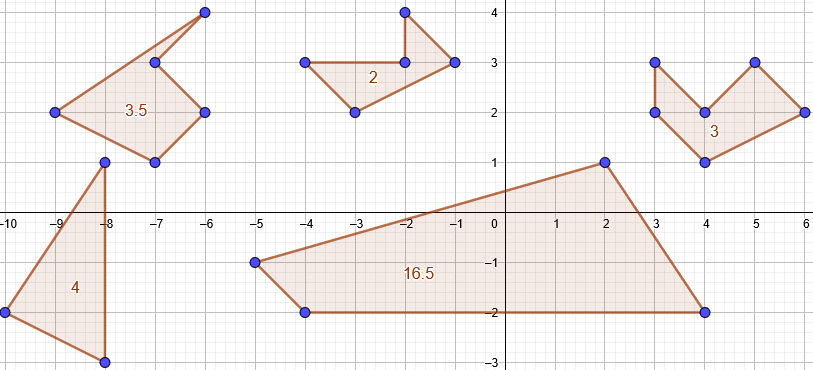
\includegraphics[width=.5\linewidth]{12}
        \end{center}
        The areas of these polygons seems to suggest area is somehow discrete, since each is either an integer, or an integer plus one-half. Area usually seems continuous, but perhaps the limited nature of this framework restricts possible areas. Moreover, every area seems to be made up of the so-called fundamental primitive triangle of area 1/2.
    \end{solution}
\end{exercise}

\begin{exercise}{13}
    Construct (at least) 5 different non-congruent primitive lattice triangles, and find their area. Make a conjecture about the value of the area of a primitive lattice triangle.
    \begin{solution}
       The triangles are shown below, along with their areas.
       
        \begin{center}
        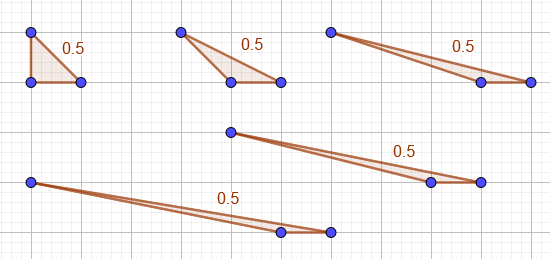
\includegraphics[width=.5\linewidth]{13}
        \end{center}
        We conjecture that all primitive triangles have the same area, 1/2. This seems to follow nicely from an ancient result by Euclid concerning triangles who share a base and whose third side lies between the same parallels.
    \end{solution}
\end{exercise}
\pagebreak
\begin{exercise}{14}
    Construct several (at least 5) different polygons that contain 4 boundary lattice points and 6 interior lattice points. Keep in mind that the polygons do not need to be convex. Find the area of each polygon. What do you observe? Make a conjecture based on your observations in this exercise.
    \begin{solution}
        The polygons, along with their areas, are shown below.
        \begin{center}
        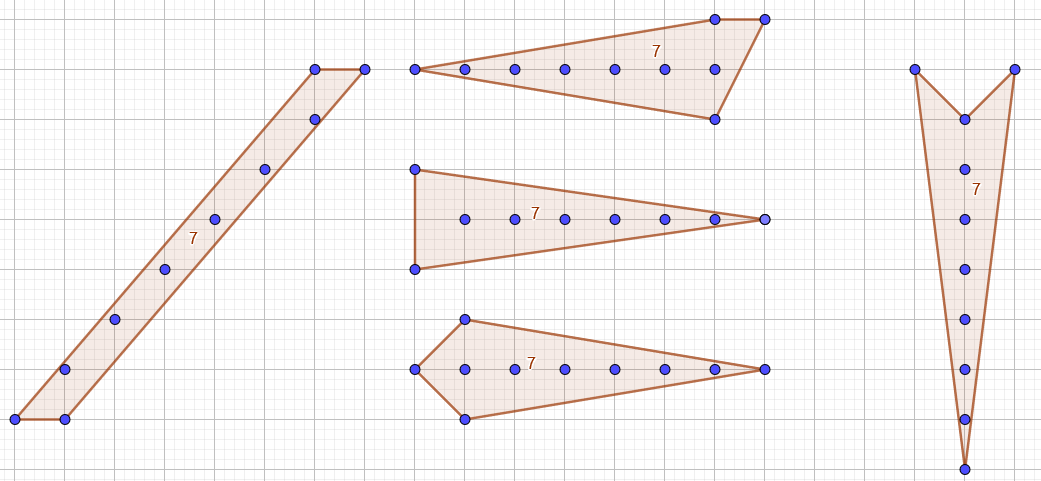
\includegraphics[width=.7\linewidth]{14}
        \end{center}
    \end{solution}
\end{exercise}\pagebreak
\begin{exercise}{15}
    Find the area of each of the lattice polygons in Figure 1. Make a table that contains the following information for each polygon: the area of the polygon, the number of lattice points inside the polygon (\( I \)), and the number of lattice points on the boundary of the polygon (\( B \)).
    \begin{solution}
        Figure 1 is shown below, and below figure 1 is a table of the areas, number of interior lattice points, and number of boundary lattice points for each polygon. Also shown is Figure 1 with each polygon partitioned into smaller polygons whose areas are easy to compute. This is how we computed area.
        \begin{center}
            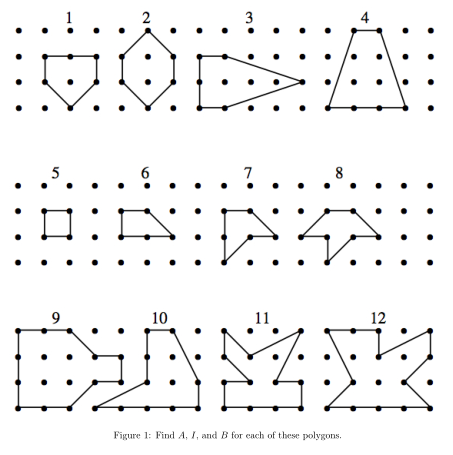
\includegraphics[width=.5\linewidth]{15}
        \end{center}
        \begin{center}
            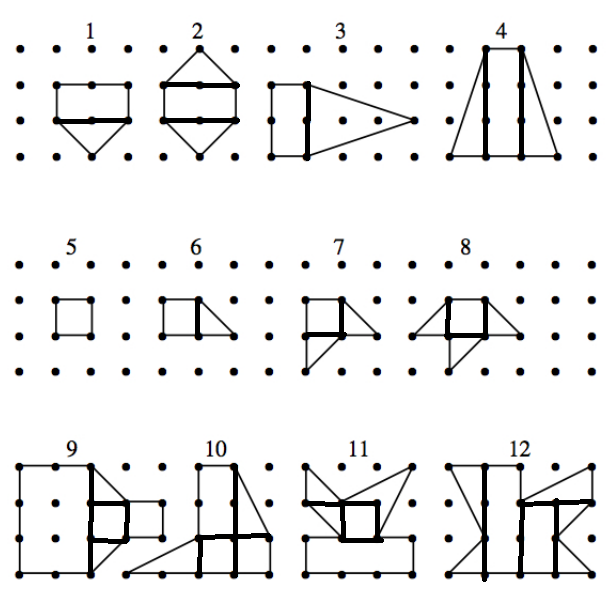
\includegraphics[width=.5\linewidth]{15-1}
        \end{center}
        \begin{center}
            \begin{tabular}{| r | l | l | l |}
                \hline
                Polygon \hspace{.75cm} & Area\hspace{1.25cm} & \( I \) \hspace{1.75cm} & \( B \) \hspace{1.75cm} \\ [.5ex]
                \hline\hline
                1 & 3 & 1 & 6\\ [3ex]
                \hline
                2 & 4 & 2 & 6\\ [3ex]
                \hline
                3 & 5 & 3 & 6\\ [3ex]
                \hline
                4 & 6 & 4 & 6\\ [3ex]
                \hline
                5 & 1 & 0 & 4\\ [3ex]
                \hline
                6 & 1/2 & 0 & 5\\ [3ex]
                \hline
                7 & 2 & 0 & 6\\ [3ex]
                \hline
                8 & 5/2 & 0 & 7\\ [3ex]
                \hline
                9 & 9 & 4 & 12\\ [3ex]
                \hline
                10 & 6 & 2 & 10\\ [3ex]
                \hline
                11 & 6 & 1 & 12\\ [3ex]
                \hline
                12 & 17/2 & 3 & 13\\ [3ex]
                \hline
                Exercise 16 \#1 & 43/2 & 16 & 13\\ [3ex]
                \hline
                Exercise 16 \#2 & 14 & 8 & 14\\ [3ex]
                \hline
                Exercise 16 \#3 & 61/2 & 21 & 21\\ [3ex]
                \hline
                Exercise 16 \#4 & 12 & 8 & 10\\ [3ex]
                \hline
                Exercise 16 \#5 & 37/2 & 14 & 11\\ [3ex]
                \hline
                Exercise 17 & 11/2 & 5 & 3\\ [3ex]
                \hline
            \end{tabular}
        \end{center}
    \end{solution}
\end{exercise}\pagebreak

\begin{exercise}{16}
    Construct 5 different lattice polygons. To keep this problem interesting, at least 3 of your polygons should be non-convex. All of your polygons should have at least 6 sides, and at least 10 boundary lattice points and at least 8 interior lattice points. For each of these 5 polygons, find the area, the number of lattice points inside the polygon, and the number of lattice points on the boundary of the polygon. Add this information to your table from Exercise 15.
    \begin{solution}
        Shown below are the five polygons satisfying the above conditions. Their information has been added to the table in exercise 15.
        \begin{center}
            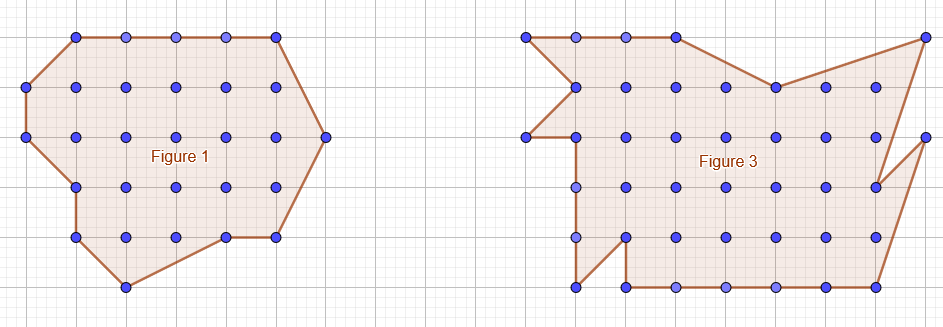
\includegraphics[width=.7\linewidth]{16-1}
        \end{center}
        \begin{center}
            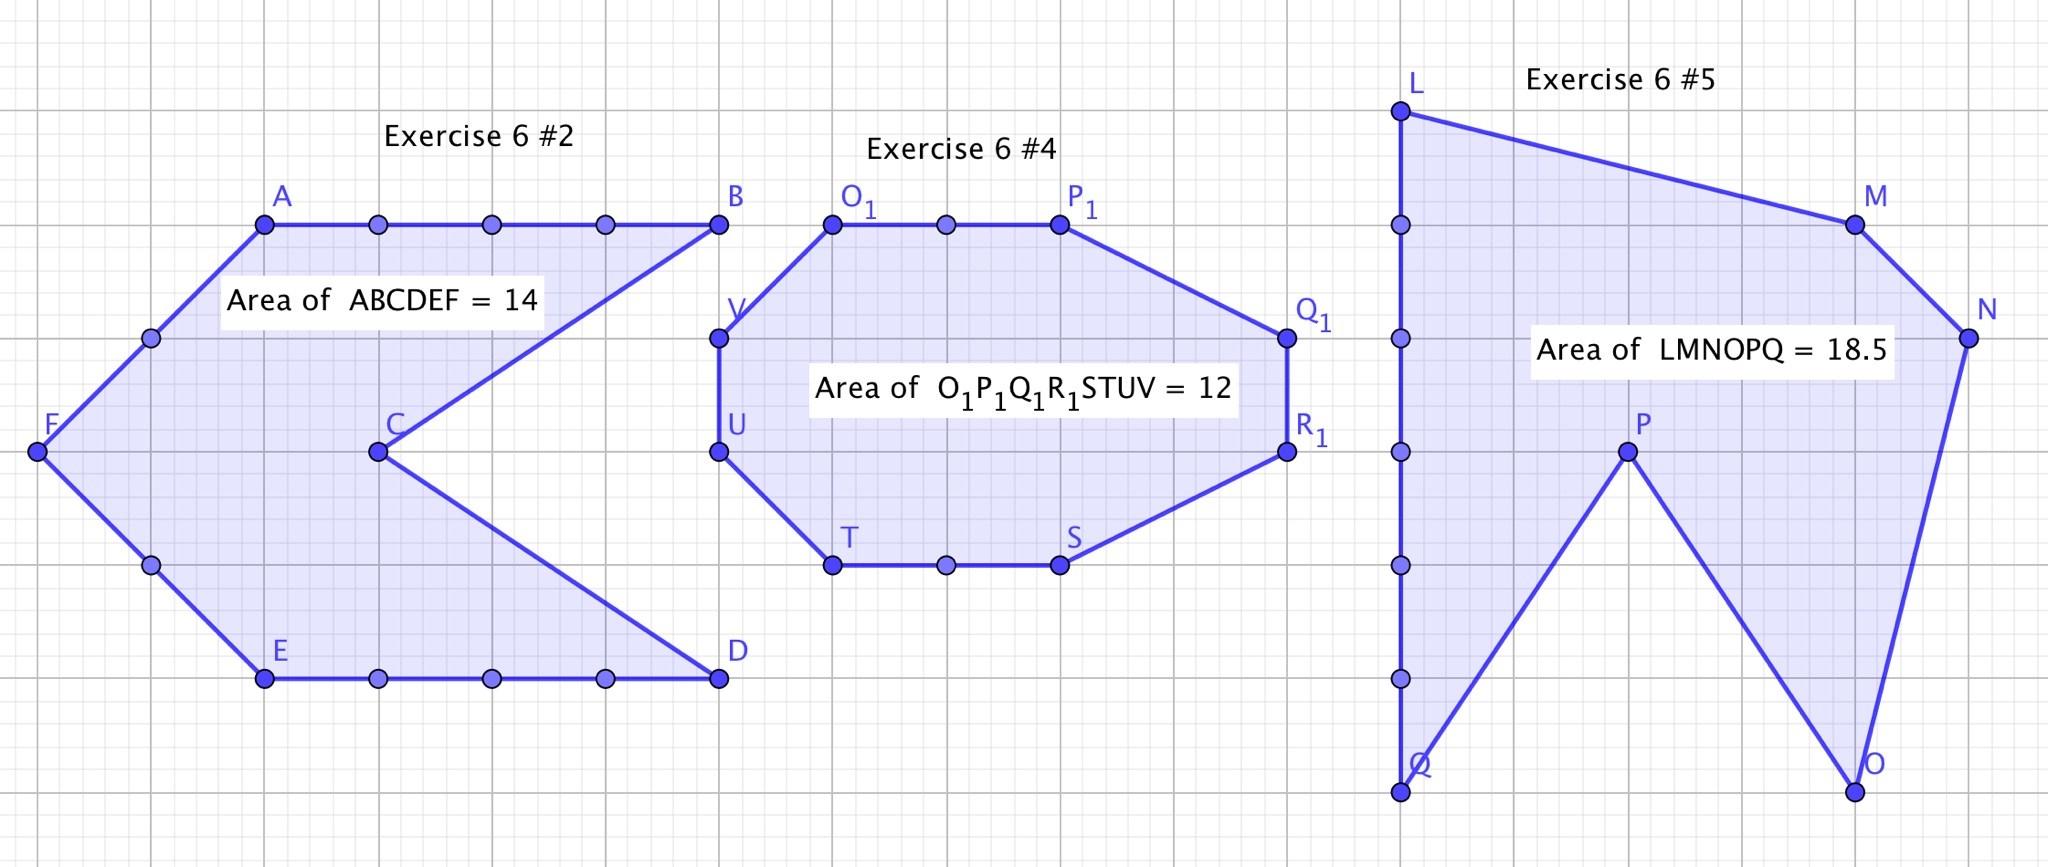
\includegraphics[width=.7\linewidth]{16-2}
        \end{center}
    \end{solution}
\end{exercise}\pagebreak

\begin{exercise}{17}
    Let \( P \) be the triangle with vertices \( ( 0,1 ) , ( 3,1 ) , \) and \( ( 1,4 ) . \) Find the area of \( P \), the number of lattice points inside the polygon, and the number of lattice points on the boundary of the polygon. Add this to information to your table from Exercise 15.
    \begin{solution}
        Shown below is the triangle. It's information has been added to the table in Exercise 15.
        \begin{center}
            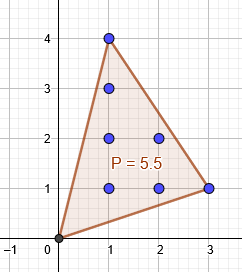
\includegraphics[width=.3\linewidth]{17}
        \end{center}
    \end{solution}
\end{exercise}

\begin{exercise}{18}
    Based on your work so far, conjecture a formula that relates the area of a lattice polygon to the number of lattice points inside the polygon and the number of lattice points on the boundary of the polygon. Explain how you obtained your conjecture, and why you think it makes sense (including a proof or partial proof if you have ideas). Although you do not need to provide a formal proof here, you should provide sufficient justification and reasoning to indicate why you believe your conjecture is valid. Please do not try to find the formula online or in another reference-it's so much more fun and interesting if you discover the formula on your own! If you're not sure where to start, start with thinking of a linear relationship. If \( I \) increases by 1 and \( B \) stays fixed, what happens to the area? Similarly, if \( B \) increases by 1 and \( I \) stays fixed, what happens to the area? Use these observations to try to find an equation that relates \( A, B, \) and \( I. \)
    \begin{solution}
        Our proposed formula for the area of a lattice polygon is:
        $$ A = I + \frac{1}{2} B -1.$$
        We arrived at this conjecture by examining the relation between various rows on the table in Exercise 15. We noticed that when the number of boundary points remained constant between polygons and the number of interior points increased by 1, then the area would increase by 1. Conversely, if the number of interior points stayed constant and the number of boundary points increased by 1, the area increased by 1/2. This led to us writing down and adjusting some equalities until we found one that generalized to all of the polygons we had worked with.

        As far as evidence to the validity of the theorem, we have a few ideas. It seems that if one takes a polygon and adds an interior point, two primitive triangles spawn. Similarly, if one adds a boundary point, it seems that one primitive triangle spawns. If this is the case, this would account for the various increases provided by adjusting boundary and interior points.
    \end{solution}
\end{exercise}

\begin{exercise}{19}
    Construct your own lattice polygon and verify that the formula that you conjectured in Exercise 18 is satisfied. Your polygon should be at least somewhat interesting-for example, make it non-convex, and have at least 10 boundary lattice points and at least 8 interior lattice points.
    \begin{solution}
        Consider the below polygon of area 17.
        \begin{center}
            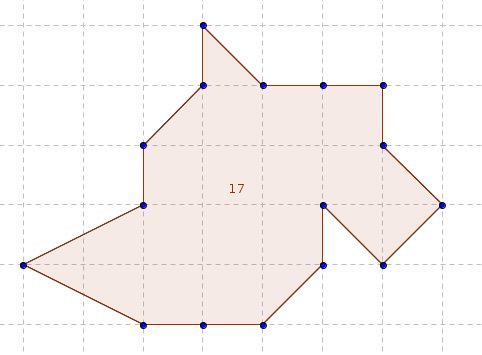
\includegraphics[width=.45\linewidth]{19}
        \end{center}
        This polygon has 16 boundary points and 10 interior points, so according to our formula,
        \begin{align*}
            A &= I + \frac{1}{2} B - 1\\
            &= 10 + \frac{1}{2} ( 16 ) - 1\\
            &= 10 + 8 - 1\\
            &= 17.
        \end{align*}
    \end{solution}
\end{exercise}

\begin{exercise}{20}
    Assuming that your conjecture in Exercise 18 is valid, make a conjecture about the possible values of the area of a lattice polygon. Explain how you obtained your conjecture, and why you think it makes sense (including a proof or partial proof if you have ideas). Although you do not need to provide a formal proof here, you should provide sufficient justification and reasoning to indicate why you believe your conjecture is valid.
    \begin{solution}
        Our formula, if true, limits the possible areas of lattice polygons. Since \( I \) and \( B \) are guaranteed to be non-negative integers (because otherwise we wouldn't have a polygon), the area is restricted to either an integer or an integer plus 1/2 (since \( A = I + 1/2B -1 \)). This is consistent with our findings.
    \end{solution}
\end{exercise}

\begin{exercise}{21}
    Does every lattice line segment have rational length? If so, prove it. If not, provide an example of a lattice line segment with non-rational length.
    \begin{solution}
        No, consider the line segment below.
        \begin{center}
            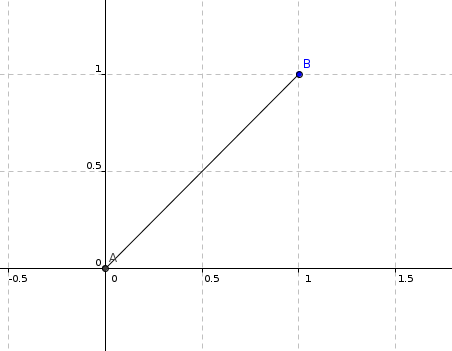
\includegraphics[width=.45\linewidth]{21}
        \end{center}
        This line segment has length \( d = \sqrt{(1-0)^{2} + ( 1 - 0 )^{2} } = \sqrt{2} \notin \Q.  \)
    \end{solution}
\end{exercise}

\begin{exercise}{22}
    Make and prove a conjecture about the square of the length of any lattice line segment.
    \begin{solution}
        We conjecture that the square of the length of any lattice line segment must be an integer. Let \( ( a,b ) , ( c,d ) \in \Z^{2} . \) Then the line segment between them has length \( d = \sqrt{( a - c )^{2} + ( b - d )^{2}} . \) Thus \( d^{2} = ( a -c )^{2} + ( b-d )^{2}, \) which is an integer since \( \Z \) is closed under addition, subtraction, and multiplication.
    \end{solution}
\end{exercise}

\begin{exercise}{23}
    Let \( L \) be a line with rational slope in the plane. Show that if there is a lattice point on \( L, \) then the \( y \)-intercept of \( L \) is rational.
    \begin{solution}
        Let \( L \) be a line with rational slope in the plane. Assume there is some lattice point \( (a,c) \) on \( L. \) Line \( L \) has slope-intercept form \( y = mx + b \) where \( m \) is the slope of \( L \) and \( b \) is the \( y \)-intercept of \( L. \) Since \( ( a,c ) \in L, \) \( c = am + b \) and \( b = c - am. \) Since \( c,m,a \in \Q \) and \( \Q \) is closed under subtraction and multiplication, \( b \in \Q. \)
    \end{solution}
\end{exercise}

\begin{exercise}{24}
    Let \( L \) be a line with rational slope in the plane. Show that if there is one lattice point on \( L, \) then there are infinitely many lattice points on \( L. \)
    \begin{solution}
        Let \( L \) be a line with rational slope in the plane. Choose \( p,q \in \Z \) such that the slope of \( L \) is \( p/q. \) Assume there is a point \( (a,c) \in \Z^{2} \) on \( L. \) Consider the point \( ( a + qn, c + pn ) \) for some \( n \in \Z^{+} . \) This point is a lattice point since \( \Z \) is closed under addition and multiplication. We will show this point satisfies the equation of line \( L. \)
        \begin{align*}
            y &= \frac{p}{q} x + b\\[.5ex]
            c &= \frac{p}{q}a + b\\[.5ex]
            c + pn &= \frac{p}{q} a + pn + b\\[.5ex]
            c + pn &= \frac{p}{q} (a + qn) + b.
        \end{align*}
        So \( ( a+qn, c+pn ) \) satisfies the equation of \( L \) and thus lies on \( L. \) Moreover, since \( \Z^{+} \) is infinite in size, we have found an infinite family of lattice points which lie on \( L. \)
    \end{solution}
\end{exercise}

\begin{exercise}{25}
    Let \( p = ( m,n ) \) be a lattice point in the plane with \( \gcd(m,n) = 1. \) Show that there are no lattice points strictly between the origin \( \mathbf{0} = ( 0,0 ) \) and \( p \) on the line segment \( \mathbf{0}p. \)
    \begin{solution}
        Assume WLOG that \( p \) is in the first quadrant of \( \Z^{2} . \) We don't lose generality by doing this, since divisibility and gcd are maintained regardless of sign.
        
        Assume for the sake of contradiction that there exists a point \( ( a,c ) \in \Z^{2} \) in between the origin and \( p \) lying on the segment \( \mathbf{0}p, \) i.e. that \( a < m \) and \( c < n. \) Since the two points lie on the same line, should be able to calculate the slop of the line in two different ways but obtain the same value.
        \begin{align*}
            \frac{n - 0}{m - 0} &= \frac{c - 0}{a - 0}\\
            \frac{n}{m} &= \frac{c}{a} .
        \end{align*}
        Cross multiplying,
        \begin{align*}
            cm = an.
        \end{align*}
        Now \( m \mid an \) since \( cm = an, \) but recall \( \gcd(m,n) = 1. \) Thus \( m \nmid n \) and \( m \mid a. \) This implies that \( m \leq a. \) Recall that \( a < m, \) and we have a contradiction. Thus there are no lattice points on \( \mathbf{0}p \) strictly in between \( p \) and \( \mathbf{0} \).
    \end{solution}
\end{exercise}

\begin{exercise}{26}
    Show that if \( p = ( m,n ) \) is a visible point on the lattice line \( L, \) then any lattice point on \( L \) is of the form \( ( tm,tn ) \) for some integer \( t. \)
    \begin{solution}
        It is important to note that a very simple proof of this exercise exists given the converse of number 25. However, we are not so easily appeased by low-hanging fruit. We proceed with our original argument, which illuminates some interesting geometric principles on the integer lattice.
        
        Assume \( p = ( m,n ) \) is a visible point on the lattice line \( L. \) Let \( t \in \Z \backslash \{ 1 \} . \) Let \( \varphi_{t}  : \R^{2} \to \R^{2} \) be the map which sends \( ( a,b ) \) to \( ( a - (t-1)m ,b - (t-1)n)  \). We will first prove that the map preserves the lattice, i.e. that \( ( x,y ) \in \Z^{2} \) if and only if \( \varphi_{t}(( x,y )) \in \Z^{2}  \). Then we will prove that the map preserves ``betweenness'', i.e. \( ( a,b ) \) lies between two points on a line if and only if \( \varphi_{t} (( a,b )) \) lies between the image of those same points on the same line.
        
        Assume \( ( a,b ) \in \Z^{2} . \) Then \( \varphi(( a,b ))_{t}  = ( a - (t-1)m, b-(t-1)n ) . \) Note that \( \Z \) is closed under subtraction and multiplication, so \( a-(t-1)m, b-(t-1)n \in \Z. \) Thus \( \varphi_{t} (( a,b )) \in \Z^{2} . \) The reverse direction is similar. Thus \( \varphi \) preserves the lattice.
        
        Now assume \( ( a,b ) \in \R^{2} \) lies on the line segment between points \((x_{1} , y_{1}) \) and \( ( x_{2} , y_{2} ) . \) We will show that \( \varphi_{t}(( a,b )) \) lies on the line segment between points \( \varphi_{t}(( x_{1} , y_{1} )) \) and \( \varphi(( x_{2} , y_{2} )) \). To do this, we rely on a well-known fact concerning the formation of triangles, namely that a point \( C \) is on a line segment \( AB \) if and only if \( AC + CB = AB. \) We will now compute the necessary distances. Let \( d_{1} \) be the distance from \( ( x_{1} , y_{1} ) \) to \( ( a,b ) \), let \( d_{2}  \) be the distance from \( ( a,b ) \) to \( ( x_{2} , y_{2} ) , \) and let \( d_{3} \) be the length of the whole line segment, or the distance from \( ( x_{1} , y_{1} ) \) to \( ( x_{2}, y_{2} ) . \) We compute these distances.
        \begin{align*}
            d_{1} &= \sqrt{( a-x_{1} )^{2} + ( b-y_{1} )^{2}} \\
            d_{2} &= \sqrt{( a-x_{2} )^{2} + ( b-y_{2} )^{2}} \\
            d_{3} &= \sqrt{( x_{1} - x_{2} )^{2} + ( y_{1} - y_{2} )^{2} } .
        \end{align*}
        By assumption, \( d_{1} + d_{2} = d_{3} . \) Now we apply \( \varphi_{t} \) to each point and compute the corresponding distances, with \( ' \) symbols indicating the translated distance.
        \begin{align*}
            d_{1}' &= \sqrt{ (a - (t-1)m - x_{1} + ( t-1 ) m)^{2} + ( b - ( t-1 ) n - y_{1} + ( t-1 ) n )^{2} }\\
             &= \sqrt{( a-x_{1} )^{2} + ( b-y_{1} )^{2}} \\
            d_{2}' &= \sqrt{ (a - (t-1)m - x_{2} + ( t-1 ) m)^{2} + ( b - ( t-1 ) n - y_{2} + ( t-1 ) n )^{2} }\\
             &= \sqrt{( a-x_{1} )^{2} + ( b-y_{1} )^{2}} \\
            d_{3}' &= \sqrt{ (x_{1} - (t-1)m - x_{2} + ( t-1 ) m)^{2} + ( y_{1}  - ( t-1 ) n - y_{2} + ( t-1 ) n )^{2} }\\
            &= \sqrt{( x_{1} - x_{2} )^{2} + ( y_{1} - y_{2} )^{2} } .
        \end{align*}
        Note that for \( i \in \{ 1,2,3 \} , d_{i} = d_{i} '.\) Thus \( d_{1} ' + d_{2} ' = d_{3}'  \) and \( \varphi_{t}(( a,b )) \) lies on the segment between \( \varphi(( x_{1} ,y_{1} ))\) and \( \varphi(( x_{2} , y_{2} )) \). The converse follows from a symmetric argument.

        We now have the machinery necessary to prove that every lattice point on the line is of the form \( ( tm, tn ) \) for some \( t \in \Z. \) Note that for all \( t \in \Z, \) \( ( tm,tn ) \) lies on the given line, since the point satisfies
        \begin{align*}
            y &= \frac{n}{m} x \\
            tn &= \frac{n}{m} tm\\
            tn &= tn.
        \end{align*}
        Consider every consecutive pair of such points: \( ( t-1 ) m, ( t-1 ) n \) and \( ( tm, tn ) . \) If \( t = 1, \) then the points are \( ( 0,0 ) \) and \( ( m,n ) , \) and we assumed that there are no lattice points on the line between these two. So, we proceed by assuming \( t\neq 1. \) Apply the map \( \varphi_{t} \) to each point to receive two new points: \( ( 0,0 ) \) and \( ( tm - (t-1)m, tn - ( t-1 )n ) = ( m,n ) . \) Recall our assumption, that there are no lattice points between \( ( 0,0 ) \) and \( ( m,n ) . \) Since \( \varphi_{t} \) preserves the lattice and betweenness, there cannot have been any lattice points between \( (( t-1 ) m, ( t-1 ) n) \) and \(( tm,tn ) .  \) We can see this by considering the result had their been such points. Let \( \mathbf{p} \) be such a point, a lattice point strictly between \( ( ( t-1 ) m, ( t-1 ) n ) \) and \( ( tm, tn ) . \) Then \( \varphi_{t}(\mathbf{p}) \) must be a lattice point between \( ( 0,0 ) \) and \( ( m,n ) , \) by the two statements we proved about \( \varphi_{t} . \) This is impossible, however, since \( ( m,n ) \) is a visible point.

        We can conclude there are no lattice points on line \( L \) between consecutive pairs of points of the form \( ( tm, tn ) . \) Thus, there are no such points on the line other than those of the form \( ( tm, tn ) \) for some \( t \in \Z. \)
    \end{solution}
\end{exercise}

\begin{exercise}{27}
    Let \( m \) and \( n \) be nonnegative integers. Show that there are exactly \( \gcd(m,n ) -1 \) lattice points on the line segment between the origin and the point \( ( m,n ) , \) not including the endpoints.
    \begin{solution}
        Assume \( m \) and \( n \) are nonnegative integers. Note that \( m \) and \( n \) cannot both be 0, since there is no segment from the origin to itself.
        
        Suppose first that \( m = 0. \) If \( m=0, \) then the line segment lies vertically on the \( y- \)axis. One can simply count the \( n-1 \) points on the vertical axis between the origin and \( ( 0,n ) , \) since they will all be of the form \( ( 0,k ) \) for \( k \in \{ 1, \ldots, n-1 \} . \) Thus there are \( n-1 \) points in this case, but we are not sure that \( \gcd(0,n) \) is even defined.
        
        Suppose now that \( n = 0. \) The result is exactly the same, except now we have a horizontally aligned segment. We simply count the points of the form \( ( k, 0 ) \) for \( k \in \{ 1, \ldots, m-1 \} \) and we have \( m-1 \) points.
        Lastly, suppose \( m \neq 0 \) and \( n\neq 0. \) Let \( d = \gcd(m,n) . \) The equation of the line through the origin and point \( ( m,n ) \) is of the form
        \begin{align*}
            y = \frac{n}{m} x.
        \end{align*}
        To reduce the fraction \( \frac{n}{m} ,\) we divide both numerator and denominator by \( d \). Let \( n = k d \) and \( m = l d. \) So the equation of the line is now
        \begin{align*}
            y = \frac{k}{l} x.
        \end{align*}
        One can check that the lattice point \( ( l, k ) \) lies on the line. Moreover, \( \gcd(l,k) = 1, \) since if they had another common factor, the \( \gcd \) of \( m \) and \( n \) would be larger. Thus \( ( l, k ) \) is visible on the line segment between the origin and \( ( m,n ) . \) Moreover, by exercise 26 we know that every lattice point on the line in question is of the form \( ( tl,tk )  \) for some \( t \in \Z. \) Note that there are exactly \( d-1 \) lattice points between \( ( l,k ) \) and \( ( m,n ) \) including \( ( l,k ) \) since \( ( m,n ) = ( dl, dk ) . \) Thus there are \( d-1 \) lattice points in between the origin and \( ( m,n ) . \)
    \end{solution}
\end{exercise}

\begin{exercise}{28}
    Let \( P \) be a lattice \( n- \)gon with vertices
    \begin{align*}
        p_{1} = ( a_{1} , b_{1} ), p_{2} = ( a_{2} , b_{2} ), \ldots , p_{n} = ( a_{n} , b_{n} ) .
    \end{align*}
    Let
    \begin{align*}
        d_{i} = \gcd ( a_{i + 1} - a_{i} , b_{i + 1} - b_{i} )
    \end{align*}
    for \( i = 1,2,\ldots,n-1 \) and let
    \begin{align*}
        d_{n} = \gcd(a_{1} - a_{n} , b_{1} - b_{n} ).
    \end{align*}
    Show that the number of lattice points on the boundary of \( P \) is given by
    \begin{align*}
        B(P) = \sum_{i=1}^nd_{i} .
    \end{align*}
    \begin{solution}
        We will use a similar method to prove this as we employed in exercise 26. Our general strategy will be to perform several translations of our polygon to the origin, in order to use the result from exercise 27. As a vehicle for this translation, consider the map
        \begin{align*}
            \varphi_{i} &: \R^{2} \to \R^{2} \\
             ( x,y ) &\mapsto ( x - a_{i} , y - b_{i} ),
        \end{align*}
        where \( i \in \{ 1, \ldots, n \} . \) Note that this map is essentially synonomous to the map developed in exercise 26, and that any integer translation of \( \R^{2} \) will exhibit the properties shown in exercise 26.

        Now consider all pairs of vertices of the polygon \( ( a_{i} , b_{i} ) \) and \( ( a_{i + 1} , b_{i+1} )  \) for \( i \in \{ 1, \ldots, n-1 \} . \) We apply \( \varphi_{i} \) to each vertex to receive new points \( ( 0,0 ) \) and \( ( a_{i + 1} - a_{i} , b_{i+1} - b_{i} ) . \) By exercise 27, there are \( d_{i} - 1 = \gcd(a_{i+1} - a_{i} , b_{i+1} - b_{i}) -1 \) lattice points strictly between the origin and our new point. By the properties of \( \varphi_{i} \) proven in exercise 26, we conclude that there are the same number of lattice points between the original points before translation: \( ( a_{i} , b_{i} ) \) and \( ( a_{i + 1} ,b_{i+1} ) . \) Now let \( i = n. \) In this case, we consider the pair of points \( ( a_{n} , b_{n} ) \) and \( ( a_{1}, b_{1} ) . \) The process is the same as before, this time applying \( \varphi_{n} . \)

        We have counted the number of points strictly between each vertex of the given polygon with \( n \) vertices. Said number is
        \begin{align*}
            \left(\sum_{i=1}^n d_{i}\right) - n.
        \end{align*}
        Since the vertices of a polygon are counted among its boundary points, we must add \( n \) to our count to account for the vertices. Thus the total number of boundary points is exactly
        \begin{align*}
            \sum_{i=1}^n d_{n} .
        \end{align*}
    \end{solution}
\end{exercise}

\begin{exercise}{29}
    \begin{enumerate}[label=(\alph*)]
        \item Is the set $$ \left\{ \begin{bmatrix}
                 1\\
                 2
        \end{bmatrix} , \begin{bmatrix}
             3\\
             4
        \end{bmatrix}\right\}  $$ a basis for \( \R^{2} ? \) Prove your result.
            \begin{solution}
                This set is a basis. Consider the matrix with columns the vectors in the set, $$ A = \begin{bmatrix}
                    1 & 3\\
                    2 & 4
                \end{bmatrix} .$$ We compute the determinant of \( A, \) \( \det(A) = 4 - 6 = -2. \) Since \( A \) has nonzero determinant, it is an invertible matrix. From linear algebra, we know that invertible matrices have as columns a basis for \( \R^{n} , \) where \( n \) is the dimension of the matrix, in this case 2. Thus the set above is a basis of \( \R^{2} . \)
            \end{solution}
        \item Is the set $$ \left\{ \begin{bmatrix}
                 1\\
                 2
        \end{bmatrix} , \begin{bmatrix}
             3\\
             4
        \end{bmatrix}\right\}  $$ a basis for \( \Z^{2} ? \) Prove your result.
            \begin{solution}
                This set is not a basis for \( \Z^{2} . \) We proceed by providing a vector in \( \Z^{2} \) which is not the result of a \( \Z \)-linear combination of the vectors in the above set. Such a vector is \( \begin{bmatrix}
                     1\\1
                \end{bmatrix}.\) Since the two integers in the second rows of each of the vectors in the set (namely 2 and 4) are even, any \( \Z \)-linear combination of those vectors will have an even number in the second row. Note that \( 1 \) is not even, and thus cannot be the second row of any \( \Z \)-linear combination of the vectors in the provided set. Thus the set does not span \( \Z^{2}  \) over \( \Z \) and is thus not a basis for \( \Z^{2} . \)
            \end{solution}
    \end{enumerate}
\end{exercise}

\begin{exercise}{30}
    Use Definition 20 to show that the matrix $$ A = \begin{bmatrix}
        1 & 3\\
        4 & 11
    \end{bmatrix}$$ is invertible over \( \Z. \)
    \begin{solution}
        According to definition 20, we wish to find a matrix \( B \) such that \( AB = I. \) Let $$ B = \begin{bmatrix}
            -11 & 3\\
            4 & -1
        \end{bmatrix} .$$ Then $$ AB = \begin{bmatrix}
            1 & 3\\
            4 & 11
        \end{bmatrix} \begin{bmatrix}
            -11 & 3\\
            4 & -1
        \end{bmatrix} = \begin{bmatrix}
            -11 + 12 & 3-3\\
            -44 + 44 & 12 -11
        \end{bmatrix} = \begin{bmatrix}
            1 & 0\\
            0 & 1
        \end{bmatrix} = I .$$
        Thus \( A \) is invertible over \( \Z. \)
    \end{solution}
\end{exercise}

\begin{exercise}{31}
    Use Definition 20 to show that the matrix $$ A = \begin{bmatrix}
        1 & 2\\
        3 & 4
    \end{bmatrix}$$ is \textit{not} invertible over \( \Z. \)
    \begin{solution}
        Suppose for the sake of contradiction that \( A \) is invertible over \( \Z. \) According to definition 20, let \( B \) be the matrix over \( \Z \) such that \( AB = I. \) Choose \( a,b,c,d \in \Z \) such that $$ B = \begin{bmatrix}
            a & b\\
            c & d
        \end{bmatrix} .$$
        Applying definition 20,
        $$ AB = \begin{bmatrix}
            1 & 2\\
            3 & 4
        \end{bmatrix} \begin{bmatrix}
            a & b\\
            c & d
        \end{bmatrix} = \begin{bmatrix}
            1 & 0\\
            0 & 1
        \end{bmatrix} = I .$$
        The matrix multiplication along with the resulting matrix yields the following equations:
        \begin{align}
            a + 2c = 1\\
            3a + 4c = 0\\
            b + 2d = 0\\
            3b + 4d = 1
        \end{align}
        Solving for \( a \) in (1), \( a = 1-2c. \) We plug \( 1-2c \) for \( a \) in (2), \begin{align*}
            3 ( 1-2c ) + 4c &=0\\
            3 - 6c + 4c &= 0\\
            3 - 2c &= 0\\
            3 &= 2c\\
            \frac{3}{2} &= c.
        \end{align*}
        But of course \( \frac{3}{2} \notin \Z. \) Thus \( c \in \Z \) and \( c \notin \Z, \) a contradiction. So \( A \) is not invertible.
    \end{solution}
\end{exercise}

\begin{exercise}{32}
    Construct at least three (non-identity) matrices with integer entries that are invertible over \( \Z. \)
    \begin{enumerate}[label=(\alph*)]
        \item Show that each of your matrices is invertible over \( \Z. \)
            \begin{solution}
                Let \( A = \begin{bmatrix}
                    3 & 4\\
                    5 & 7
                \end{bmatrix} , B = \begin{bmatrix}
                    5 & 2\\
                    2 & 1
                \end{bmatrix} ,\) and \( C = \begin{bmatrix}
                    1 & 1\\
                    5 & 4
                \end{bmatrix} .\)
                To show that each matrix is invertible over \( \Z, \) we will find an inverse for each in \( M_{2}(\Z) . \) Let \( A' = \begin{bmatrix}
                    7 & -4\\
                    -5 & 3
                \end{bmatrix}, B' = \begin{bmatrix}
                    1 & -2\\
                    -2 & 5
                \end{bmatrix} , \) and \( C' = \begin{bmatrix}
                    -4 & 1\\
                    5 & -1
                \end{bmatrix} .\) Quick computations show that \( AA' = I, \) \( BB' = I, \) and \( CC' = I. \)
            \end{solution}
        \item Find the determinant of each of your matrices. What do you observe?
            \begin{solution}
                We see that \( \det(A) = 1, \det(B) = 1, \) and \( \det(C) = -1. \) They are all \( \pm 1. \)
            \end{solution}
        \item Performing additional computations if necessary, make a conjecture about the determinant of a matrix with integer entries that is invertible over \( \Z \).
            \begin{solution}
                We conjecture that the determinant of such matrices is either 1 or \( -1. \)
            \end{solution}
    \end{enumerate}
\end{exercise}

\begin{exercise}{33}
    \begin{enumerate}[label=(\alph*)]
        \item  Let \( A \) be a matrix with entries in \( \R . \) Complete the following statement: \( A \) is invertible (over \( \R \)) if and only if \( \det(A) \ \rule{2cm}{0.15mm}  \). Note: you do not need to prove this result here; you simply need to recall the appropriate result from linear algebra.
            \begin{solution}
                The blank should be \( \det(A) \neq 0. \)
            \end{solution}
        \item State the formula for the inverse \( A^{-1} \) of an invertible matrix $$ \begin{bmatrix}
                a & c\\
                b & d
        \end{bmatrix}$$ with entries in \( \R. \) How is this result consistent with your statement from part (a) of this problem?
            \begin{solution}
                Recall the classic formula
                $$ \frac{1}{\det(A)} \begin{bmatrix}
                    d & -c\\
                    -b & a
                \end{bmatrix} .$$ This is consistent with our statement from part (a) since division by 0 is undefined over \( \R. \)
            \end{solution}
    \end{enumerate}
\end{exercise}

\begin{exercise}{34}
    Let \( A \) be a 2x2 matrix with entries in \( \Z. \) Show that \( A \) is invertible over \( \Z \) if and only if \( \det(A) = \pm 1. \) Note that you only need to prove this result here for \( 2x2 \) matrices, but the same result holds for more general \( n \times n \) matrices with entries in \( \Z. \) (You are of course welcome to prove the more general result here, if you wish.)
    \begin{solution}
        Assume \( A \) is invertible over \( \Z. \) By definition 20, there is a \( B \in M_{2}(\Z) \) such that \( AB = I. \) By familiar properties of the determinant, \( \det(AB) = \det(A) \det(B) . \) Since \( AB = I, \) \( \det(A) \det(B) = 1. \) We claim that the determinant of a \( 2 \times 2 \) matrix with entries in \( \Z \) must be an integer. To see this, consider the matrix \( \begin{bmatrix}
            a & b\\
            c & d
        \end{bmatrix} \) with determinant \( ad - bc. \) Since \( \Z \) is closed under multiplication and subtraction, the determinant must be an integer. Thus \( \det(A) \) and \( \det(B) \) are integers. The only integers who multiply to 1 are 1 and \( -1. \) Thus \( \det(A) = \pm 1. \)\\
        Conversely, assume that \( \det(A) = \pm 1. \) Choose \( a,b,c,d \in \Z \) such that \( A = \begin{bmatrix}
            a & b\\
            c & d
        \end{bmatrix} .\) Let \( B =
            \ds\frac{1}{\det(A)} \begin{bmatrix}
                d & -b\\
                -c & a
            \end{bmatrix}\) A quick computation will show that \( AB = I. \) Now since \( \det(A) = \pm 1 , B = \begin{bmatrix}
                d & -b\\
                -c & a
            \end{bmatrix}\) or \( B = \begin{bmatrix}
                -d & b\\
                c & -a
            \end{bmatrix} .\) In both cases, \( B \in M_{2}(\Z) . \) Thus \( A \) is invertible over \( \Z. \)
    \end{solution}
\end{exercise}

\begin{exercise}{35}
    Which real numbers have multiplicative inverse in \( \R? \) Prove your result.
    \begin{solution}
        All nonzero real numbers have multiplicative inverse in \( \R. \) Let \( a \in \R \backslash \{0\} \). Then \( 1/a \in \R. \) Thus \( a \) has a multiplicative inverse in \( \R. \)
    \end{solution}
\end{exercise}

\begin{exercise}{36}
    Which \textit{integers} have a multiplicative inverse that is \textit{also an integer}? Prove your statement.
    \begin{solution}
        Only \( \pm 1 \) have integer multiplicative inverses in \( \Z. \) Let \( a \in \Z \backslash \{-1,1\} \). Suppose there is a \( b \in \Z \) such that \( ab = 1. \) Then \( b = 1/a. \) But \( 1/a \notin \Z \) for all \( a \in \Z\backslash \{ -1,1 \} . \) Thus \( a \) has no multiplicative inverses in \( \Z. \)
    \end{solution}
\end{exercise}

\begin{exercise}{37}
    Observe that Exercise \( 33 \)(a) implies that a matrix \( A \) with entries in \( \R \) is invertible over \( \R \) if and only if \( \det(A) \) has a multiplicative inverse in \( \R. \) Use the results of the previous exercises to show that a matrix \( A \) with entries in \( \Z \) is invertible over \( \Z \) if and only if \( \det(A) \) has a multiplicative inverse which is also an integer. This exercise provides a beautiful connection between invertibility of a matrix with entries in a given space and invertibility of the determinant of the matrix in that space.
    \begin{solution}
        By exercise 36, the only integers whose multiplicative inverse is also an integer are \( \pm1. \) Thus, we change the consequent of 34 with an equivalent statement to find that a matrix \( A \) with entries in \( \Z \) is invertible over \( \Z \) if and only if \( \det(A) \) has a multiplicative inverse which is also an integer.
    \end{solution}
\end{exercise}

\begin{exercise}{38}
    Construct 3 different examples of \( \Z \)-bases \( \{ \mathbf{v} = \langle v_{1} , v_{2} \rangle , \mathbf{w} = \langle w_{1} , w_{2} \rangle \} \) of \( \Z^{2} . \)
    \begin{enumerate}[label=(\alph*)]
        \item Show that each of your examples is actually a \( \Z \)-basis of \( \Z^{2} . \)
            Let \( A = \{ \langle 4,3 \rangle , \langle 1,1 \rangle \} . \) We wish to show these vectors are \( \Z \)-linearly independent. Suppose there exist \( c_{1} , c_{2} \in \Z \) such that \( \langle 4,3 \rangle c_{1} + \langle 1,1 \rangle c_{2} = \langle 0,0 \rangle . \) We set up the augmented coeffictient matrix for \( c_{1} \) and \( c_{2} . \)
            \begin{align*}
                \begin{amatrix}{2}
                4 & 1 & 0\\
                3 & 1 & 0
                \end{amatrix} \xRightarrow{I - II}
                \begin{amatrix}{2}
                1 & 0 & 0\\
                3 & 1 & 0
                \end{amatrix}\xRightarrow{II - 3I}
                \begin{amatrix}{2}
                1 & 0 & 0\\
                0 & 1 & 0
                \end{amatrix}
            \end{align*}
            So \( \langle c_{1} , c_{2} \rangle = \langle 0,0 \rangle \) is the only solution and the vectors in \( A \) are \( \Z \)-linearly independent. We will now show \( A \) spans \( \Z^{2} . \) Let \( \langle a,b\rangle \in \Z^{2}  \) be an arbitrary vector. We wish to solve the equation \( \langle 4,3 \rangle c_{1} + \langle 1,1 \rangle c_{2} = \langle a,b \rangle  \) for integers \( c_{1} \) and \( c_{2} . \) We set up the augmented coefficient matrix for \( c_{1} \) and \( c_{2} . \)
            \begin{align*}
                \begin{amatrix}{2}
                4 & 1 & a\\
                3 & 1 & b
                \end{amatrix} \xRightarrow{I - II}
                \begin{amatrix}{2}
                1 & 0 & a-b\\
                3 & 1 & b
                \end{amatrix}\xRightarrow{II - 3I}
                \begin{amatrix}{2}
                1 & 0 & a-b\\
                0 & 1 & 4b-3b
                \end{amatrix}
            \end{align*}
            Thus \( c_{1} = a-b \in \Z \) and \( c_{2} = 4b-3b \in \Z \) solve the equation. So \( A \) \( \Z \)-spans \( \Z^{2} . \)

            Let \( B = \{ \langle 1,3 \rangle , \langle 2,7 \rangle \} . \) We will show \( B \) is \( \Z \)-linearly independent. Again, we wish to solve the equaion \( \langle 1,3 \rangle c_{1} + \langle 2,7 \rangle c_{2} = \langle 0,0 \rangle .\) We form the augmented coefficient matrix for \( c_{1} \) and \( c_{2} . \)
            $$ \begin{amatrix}{2}
                1 & 2 & 0\\
                3 & 7 & 0
            \end{amatrix}\xRightarrow{II - 3I} \begin{amatrix}{2}
                1 & 2 & 0\\
                0 & 1 & 0
            \end{amatrix} \xRightarrow{I-2I}
            \begin{amatrix}{2}
                1 & 0 & 0\\
                0 & 1 & 0
            \end{amatrix} .$$
            So \( \langle c_{1} , c_{2} \rangle = \langle 0,0 \rangle \) is the only solution and the vectors in \( B \) are \( \Z \)-linearly independent. We move to show the vectors span \( \Z^{2} . \) Let \( \langle a,b \rangle \in \Z^{2} \) be arbitrary. We wish to solve the equation \( \langle 1,3 \rangle c_{1} + \langle 2,7 \rangle c_{2} = \langle a,b \rangle \) for integers \( c_{1} \) and \( c_{2} . \) We form the augmented coefficient matrix for \( c_{1} \) and \( c_{2} . \)
            $$ \begin{amatrix}{2}
                1 & 2 & a\\
                3 & 7 & b
            \end{amatrix}\xRightarrow{II - 3I} \begin{amatrix}{2}
                1 & 2 & a\\
                0 & 1 & b-3a
            \end{amatrix} \xRightarrow{I-2I}
            \begin{amatrix}{2}
                1 & 0 & 7a - 2b\\
                0 & 1 & b-3a
            \end{amatrix} .$$
            Thus \( \langle c_{1} , c_{2} \rangle = \langle 7a - 2b , b-3a \rangle \in \Z^{2} \) solves the equation and \( B \) \( \Z \)-spans \( \Z^{2} . \)

            Let \( C = \{ \langle 3,2 \rangle , \langle 8,5 \rangle \} . \) We will show \( C \) is \( \Z \)-linearly independent. Again, we wish to solve the equaion \( \langle 3,2 \rangle c_{1} + \langle 8,5 \rangle c_{2} = \langle 0,0 \rangle .\) We form the augmented coefficient matrix for \( c_{1} \) and \( c_{2} . \)
            $$ \begin{amatrix}{2}
                3 & 8 & 0\\
                2 & 5 & 0
            \end{amatrix} \xRightarrow{I-II}
            \begin{amatrix}{2}
                1 & 3 & 0\\
                2 & 5 & 0
            \end{amatrix} \xRightarrow{II-2I}
            \begin{amatrix}{2}
                1 & 3 & 0\\
                0 & -1 & 0
            \end{amatrix} \xRightarrow{I + 3II \text{ and } -1\cdot II}
            \begin{amatrix}{2}
                1 & 0 & 0\\
                0 & 1 & 0
            \end{amatrix}.$$
            Thus the only solution is \( \langle c_{1} , c_{2} \rangle = \langle 0,0 \rangle  \) and the vectors in \( C \) are \( \Z \)-linearly independent. We will now show the vectors \( \Z \)-span \( \Z^{2} . \) Let \( \langle a,b \rangle \in \Z^{2} \) be an arbitrary vector. We wish to solve the equation \( \langle 3,2 \rangle c_{1} + \langle 8,5 \rangle c_{2} = \langle a,b \rangle \) for integers \( c_{1} \) and \( c_{2} . \) We form the augmented coefficient matrix for \( c_{1} \) and \( c_{2} . \)
            $$ \begin{amatrix}{2}
                3 & 8 & a\\
                2 & 5 & b
            \end{amatrix} \xRightarrow{I-II}
            \begin{amatrix}{2}
                1 & 3 & a-b\\
                2 & 5 & b
            \end{amatrix} \xRightarrow{II-2I}
            \begin{amatrix}{2}
                1 & 3 & a-b\\
                0 & -1 & 3b-2a
            \end{amatrix} \xRightarrow{I + 3II \text{ and } -1\cdot II}
            \begin{amatrix}{2}
                1 & 0 & 10a - 7b\\
                0 & 1 & 2a-3b
            \end{amatrix}.$$
            Thus \( \langle c_{1} , c_{2} \rangle = \langle 10a-7b, 2a-3b \rangle \in \Z^{2} \) solves the equation and so \( B \) \( \Z \)-spans \( \Z^{2} . \)

            Since each of \( A, B, \) and \( C \) contain \( \Z \)-linearly independent vectors which span \( \Z^{2} \) using only integer scalars, \( A,B, \) and \( C \) form bases for \( \Z^{2} . \)
        \item For each basis, compute the determinant of the matrix $$ \begin{bmatrix}
                v_{1} & w_{1}\\
                v_{2} & w_{2}
        \end{bmatrix} .$$ What do you observe?

        \begin{solution}
            We applied the determinant formula \( v_{1} w_{2} - w_{1} v_{2} \) to find determinants of 1, 1, and \( -1 \) for the matrices formed from \( A, B, \) and \( C \) respectively. It seems like the only possible determinants for such matrices are \( \pm 1. \)
        \end{solution}
    \item Doing more computations if necessary, state and prove a conjecture about the determinant of a matrix whose columns form a \( \Z \)-basis for \( \Z^{2} \).
        \begin{solution}
            We conjecture that the columns of a matrix in \( M_{2}(\Z) \) form a \( \Z \)-basis for \( \Z^{2} \) if and only if the determinant of that matrix is \( \pm 1. \)

            Assume that the columns of \( A = \begin{bmatrix}
                a_{1} & a_{2} \\
                b_{1} & b_{2}
            \end{bmatrix}\in M_{2}(\Z)  \) form a \( \Z \)-basis for \( \Z^{2} . \) Note that the columns of the identity matrix form a \( \Z \)-basis for \( \Z^{2} . \) By Theorem 1, there exists an \( L \in M_{2}(\Z) \) such that \( L \) is invertible and $$ A = L I = L. $$ Multiplying my \( L^{-1} \) on the right of both sides yields $$ A L^{-1} = I . $$ Thus \( A \) is an invertible matrix over \( \Z. \) By exercise 34, \( \det(A) = \pm 1. \)

            Conversely, assume that the determinant of a matrix \( A = \begin{bmatrix}
                a & b \\
                c & d
            \end{bmatrix} \) with integer entries is \( \pm 1. \) We will first show that the columns of \( A \) are \( \Z \)-linearly independent. Since the determinant of \( A \) is nonzero, \( A \) is invertible over \( \R. \) Since \( A \) is invertible over \( \R, \) the columns of \( A \) are linearly independent over \( \R. \) Since \( \Z \subseteq \R, \) there are no integer solutions to the equation \( \langle a,c \rangle c_{1} + \langle b,d \rangle c_{2} = \langle 0,0 \rangle \) other than the trivial solution. Thus the columns of \( A \) are \( \Z \)-linearly independent.

            We will now show that the columns of \( A \) span \( \Z^{2} . \) Let \( \langle e,f \rangle \in \Z^{2} \) be arbitrary. We wish to find integers \( c_{1} \) and \( c_{2} \) such that \( \langle a,c \rangle c_{1} + \langle b,d \rangle c_{2} = \langle e,f \rangle . \) This yields equations,
            \begin{align*}
                ac_{1} + b c_{2} &= e\\
                c c_{1} + d c_{2} &= f.
            \end{align*}
            Multiplying the top equation by \( -c  \) and the bottom equation by \( a , \)
            \begin{align*}
                -acc_{1} - bcc_{2} &= -ec\\
                acc_{1} + adc_{2} &= af.
            \end{align*}
            Adding,
            \begin{align*}
                c_{2} ( ad-bc ) = af - ec.
            \end{align*}
            Since \( \det(A) = ad-bc = \pm 1 \) by assumption, \( c_{2} = \pm (af-ec) \in \Z. \) Similar computations will show that \( c_{1} = \pm ( de - bf ) \in \Z  . \) Thus we have found integers \( c_{1} \) and \( c_{2} \) which satisfy \( \langle a,c \rangle c_{1} + \langle b,d \rangle c_{2} = \langle e,f \rangle . \) So the columns of \( A \) span \( \Z^{2} . \) Thus the columns form a \( \Z \)-basis for \( \Z^{2} . \)
        \end{solution}
    \end{enumerate}
\end{exercise}\pagebreak
\begin{exercise}{39}
    Sketch the parallelogram spanned by each of the bases that you constructed in Exercise 38.
    \begin{center}
        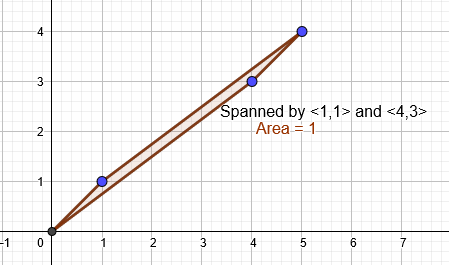
\includegraphics[width=.5\linewidth]{39-2}
        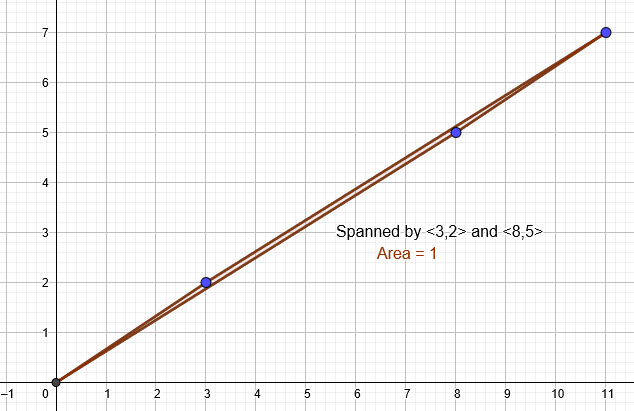
\includegraphics[width=.5 \linewidth]{39-1}
        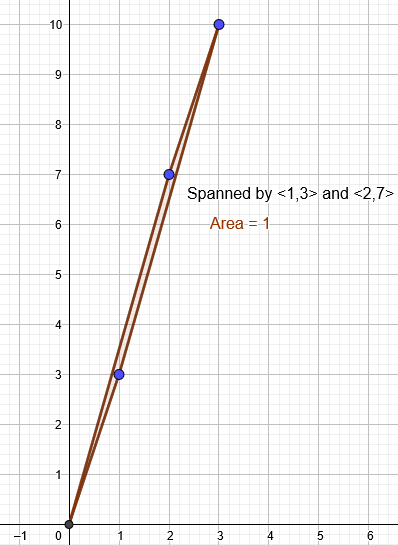
\includegraphics[width=.4\linewidth]{39-3}
    \end{center}
    \begin{enumerate}[label=(\alph*)]
        \item Find the area of the parallelogram spanned by each of the bases that you constructed in Exercise 38.
            \begin{solution}
                The area of each parallelogram is 1.
            \end{solution}
        \item State and prove a conjecture about the area of a lattice parallelogram \( P(\mathbf{v,w}) \) where \( \mathbf{v} \) and \( \mathbf{w} \) form a basis of \( \Z^{2}. \)
            \begin{solution}
                Our conjecture is that the parallelogram spanned by vectors
                which form a \( \Z \)-basis for \( \Z^{2} \) will have area 1.
                Assume \( \{\mathbf{v} , \mathbf{w}\} \) \( \subset \Z^{2} \) forms a \(
                \Z \) basis for \( \Z^{2} . \) Choose \( v_{1} , v_{2} ,
                w_{1} , w_{2} \in \Z \) such that \( \mathbf{v} = \langle v_{1}
                , v_{2}\rangle \) and \( \mathbf{w} = \langle w_{1} , w_{2}
                \rangle \) . We can project \( \mathbf{v} \) and \( \mathbf{w}\) into \( \R^{3} \) via the linear map \( T : \R^{2} \to \R^{3},  \) which sends an arbitrary vector \( \langle x,y \rangle \) to \( \langle x,y,0 \rangle . \) Recall the convenient fact that the area of the parallelogram spanned by two vectors in \( \R^{3} \) is equal to the magnitude of the cross product between the two vectors. Using the result from exercise 38, we compute
                \begin{align*}
                    \left| \langle v_{1} , v_{2} , 0 \rangle \times\langle w_{1} , w_{2} , 0\rangle  \right| &= \left|\det\left(
                    \begin{bmatrix}
                        \mathbf{i} & \mathbf{j} & \mathbf{k} \\
                        v_{1} & w_{1} & 0\\
                        v_{2} & w_{2} & 0
                    \end{bmatrix}
                \right) \right|\\
                    &= \left| \mathbf{i} \det \left(
                    \begin{bmatrix}
                        w_{1} & 0\\
                        w_{2} & 0\\
                    \end{bmatrix}
                    \right) - \mathbf{j} \det \left(
                    \begin{bmatrix}
                        v_{1} & 0\\
                        v_{2} & 0\\
                    \end{bmatrix}
                    \right) + \mathbf{k} \det \left(
                    \begin{bmatrix}
                        v_{1} & w_{1} \\
                        v_{2} & w_{2}
                    \end{bmatrix}
                \right)\right|\\
                    & = \left|\langle 0, 0, v_{1}w_{2} - w_{1} v_{2} \rangle\right| \\
                    &= \left|\langle 0, 0, \det \left(
                    \begin{bmatrix}
                        v_{1} & w_{1} \\
                        v_{2} & w_{2}
                    \end{bmatrix}
                    \right) \rangle \right|\\
                    &=\left| \langle 0,0,\pm 1 \rangle\right|\\
                    &= 1.
                \end{align*}
            \end{solution}
    \end{enumerate}
\end{exercise}

\begin{exercise}{40}
    Sketch the parallelogram spanned by each of the bases that you constructed in Exercise 38.
    \begin{enumerate}[label=(\alph*)]
        \item How many lattice points are on the sides of the parallelogram. How many lattice points are on the interior?
            \begin{solution}
                The only lattice points in the parallelograms are the boundary points.
            \end{solution}
        \item Doing more computations if necessary, make and prove a conjecture about the number of lattice points on the sides and in the interior of a lattice parallelogram \( P(\mathbf{v,w}) \) where \( \mathbf{v} \) and \( \mathbf{w} \) form a basis of \( \Z^{2}. \)
            \begin{solution}
                We conjecture that the parallelogram spanned by \( \mathbf{v} \) and \( \mathbf{w} \) has no lattice points (on the sides or on the edges) other than the vertices.

                Suppose for the sake of contradiction that there is a vector \( \mathbf{u} \in \Z^{2}  \) in the parallelogram spanned by \( \mathbf{v} \) and \( \mathbf{w} \) (either on the sides or on the edges). Since \( \mathbf{v} \) and \( \mathbf{w} \) span \( \Z^{2} , \) there exist integers \(c_{1} \) and \( c_{2} \) such that \( c_{1} \mathbf{v} + c_{2} \mathbf{w} = \mathbf{u}  \). Also, since \( \mathbf{u} \in P ( \mathbf{v} , \mathbf{w}) \), there exist real numbers \( x, y \) such that \( 0 \leq x,y \leq 1 \) and \( x \mathbf{v} + y \mathbf{w} = \mathbf{u} . \) Subtracting each of these equations,
                \begin{align*}
                    (x - c_{1}) \mathbf{v} + (y - c_{2}) \mathbf{w} = \mathbf{0} .
                \end{align*}
                Since \( \mathbf{v} \) and \( \mathbf{w} \) span \( \Z^{2} , \) by a previous exercise, the determinant of the matrix whose columns are \( \mathbf{v} \) and \( \mathbf{w} \) is \( \pm 1 \neq 0. \) Thus the same matrix is invertible over \( \R, \) and its columns form a basis for \( \R^{2} . \) Thus \( \mathbf{v} \) and \( \mathbf{w} \) are \( \R \)-linearly independent, and
                \begin{align*}
                    x - c_{1} &= 0\\
                    y-c_{2} &= 0.
                \end{align*}
                So \( c_{1} = x \) and \( c_{2} = y. \) Since \( c_{1} \) and \( c_{2} \) are integers, and \( 0 \leq x,y \leq 1, \) \( c_{1}, c_{2} \in \{0,1 \} . \) Each of the four possibilities force \( \mathbf{u} \) to be a vertex of \( P(\mathbf{v} , \mathbf{w}) . \)
            \end{solution}
    \end{enumerate}
\end{exercise}

\begin{exercise}{41}
    Suppose that the parallelogram \( P(\mathbf{v, w}) , \) where \( \mathbf{v,w} \in \Z^{2} \), is a primitive lattice parallelogram. Show that \( \mathbf{v} \) and \( \mathbf{w} \) form a basis for \( \Z^{2} . \)
    \begin{solution}
        We will first show \( \mathbf{v} \) and \( \mathbf{w} \) are \( \Z \)-linearly independent. Since \( \mathbf{v} \) and \( \mathbf{w} \) form a nondegenerate parallelogram, they cannot span the same line. Thus \( \mathbf{v} \) and \( \mathbf{w} \) are both \( \Z \)-linearly independent and \( \R \)-linearly independent.

        Now we will show \( \mathbf{v} \) and \( \mathbf{w} \) span \( \Z^{2} . \) Let \( \mathbf{u} \in \Z^{2} \) be arbitrary. Since \( \mathbf{v} \) and \( \mathbf{w} \) are two \( \R \)-linearly independent vectors in \( \R^{2} , \) they form a basis for \( \R^{2} . \) Choose \( \alpha , \beta \in \R \) such that \( \alpha \mathbf{v} + \beta \mathbf{w} = \mathbf{u} . \) Consider the vector
        \begin{align*}
            \mathbf{u'} &= \left( \alpha - \lfloor \alpha \rfloor \right) \mathbf{v} + \left( \beta - \lfloor \beta \rfloor   \right)\mathbf{w} \\
        \end{align*}
        Note that \(0 \leq   \alpha - \lfloor \alpha \rfloor < 1 \) and \( 0 \leq \beta - \lfloor \beta \rfloor <  1  \) by definition of floor. Thus \( \mathbf{u'} \in P(\mathbf{v} , \mathbf{w}) \). Also, since \( \lfloor \alpha \rfloor , \lfloor \beta \rfloor \in \Z \) and \( \mathbf{u} \in \Z^{2} , \)
        \begin{align*}
            \mathbf{u'} = \mathbf{u} - \lfloor \alpha \rfloor \mathbf{v} - \lfloor \beta \rfloor \mathbf{w} \in \Z^{2}.
        \end{align*}
        So \( \mathbf{u'} \in \Z^{2} \) and \( \mathbf{u'} \in P(\mathbf{v} , \mathbf{w}) . \) Since \( P(\mathbf{v} , \mathbf{w}) \) is primitive, the only lattice points it contains are its vertices. Thus \( \alpha - \lfloor \alpha \rfloor = \beta - \lfloor \beta \rfloor = 0, \) since each is strictly less than 1. Thus, \(\alpha\) and \(\beta\) are equal to their floor, meaning they have no decimal component. Thus \( \alpha , \beta \in \Z \) and \( \mathbf{v} \) and \( \mathbf{w} \) span \( \Z^{2} . \)
    \end{solution}
\end{exercise}

\begin{exercise}{42}
    Let \( T \) be a primitive lattice triangle. If \( \mathbf{v} \) and \( \mathbf{w} \) are vectors corresponding to adjacent sides of \( T , \) show that \( \mathbf{v} \) and \( \mathbf{w} \) form a \( \Z \)-basis of \( \Z^{2} . \)
    \begin{solution}
        Our approach to this problem involves creating a primitive lattice parallelogram based on the vectors \( \mathbf{v} \) and \( \mathbf{w}  \), and then using exercise 41 to conclude \( \mathbf{v} \) and \( \mathbf{w} \) form a \( \mathbb{Z} \)-basis for \( \mathbb{Z}^{2} . \) Consider the parallelogram spanned by \( \mathbf{v} \) and \( \mathbf{w} , \) whose vertices are \( (0,0) , (v_{1} , v_{2}) , (w_{1} , w_{2}) , \) and \( (v_{1} + w_{1} , v_{2} + w_{2}) . \) We will now show \( P(\mathbf{v} , \mathbf{w}) \) is primitive.

        The additional area of the parallelogram added on to \( T \) is simply a copy of \( T \) which has been rotated about the midpoint of the far side of the triangle. We wish to show that the transformations required to relate the two shapes preserve the lattice and actually send points to the correct shape.

        Consider the map
        \begin{align*}
            &\varphi : \mathbb{R}^{2} \to \mathbb{R}^{2} \\
            &(x,y) \mapsto (x - \frac{1}{2} (v_{1} + w_{1}) , y - \frac{1}{2} (v_{2} + w_{2})) .
        \end{align*}
        Note that this map is invertible, with inverse
        \begin{align*}
            &\varphi^{-1}  : \mathbb{R}^{2} \to \mathbb{R}^{2} \\
            &(x,y) \mapsto (x + \frac{1}{2} (v_{1} + w_{1}) , y + \frac{1}{2} (v_{2} + w_{2})) .
        \end{align*}
        Consider also the linear map given by the matrix
        \begin{align*}
            R : \mathbb{R}^{2} \to \mathbb{R}^{2} \\
            R =
            \begin{bmatrix}
                -1 & 0\\
                0 & -1
            \end{bmatrix}
        \end{align*}
        The map which will represent our transformation is \( T = \varphi^{-1} R \varphi . \) What in the world? Well, basically we want to translate the parallelogram so that the midpoint of the diagonal of the parallelogram is the origin, then we want to use Linear Algebra to rotate the plane by \( \pi \) radians, then we want translate the figure back to its original position. Let the upper triangle be herein referred to as \( T_{2} , \) and the original triangle as \( T_{1} \). We need to show two things:
        \begin{enumerate}
            \item A point \( (x, y) \in \mathbb{Z}^{2} \) if and only if \( T((x ,y)) \in \mathbb{Z}^{2} . \) This is not immediately obvious since we are adding non-integers to integers in our maps.
            \item A point \( (x,y) \in T_{2} \) if and only if \( T((x,y)) \in T_{1} . \) Chad, you might say, why not set up the maps so that you start in \( T_{1} \) and end in \( T_{2} ? \) Well, curious reader, I didn't think of that until now, and I don't really want to rework the problem.
        \end{enumerate}
        We will begin by proving 1. Let \( (x , y) \in \mathbb{Z}^{2} . \) A quick computation shows that \( T((x,y)) = (v_{1} + w_{1} - x, v_{2} + w_{2} - y) . \) Now \( v_{1} ,w_{1} , v_{2} , \) and \( w_{2} \) are all integers since they are coordinates of the vertices of our starting lattice triangle. The integers are closed under addition and subtraction, so \( T((x,y)) \in \Z^{2} . \)

        Conversely, suppose that \( T((x , y)) = (v_{1} + w_{1} - x , v_{2} + w_{2} - y) \in \Z^{2} . \) Choose \( t \in \Z \) such that \( v_{1} + w_{1} - x = t. \) So \( x = v_{1} + w_{1} -t \in \Z. \) Similarly, \( y \in \Z. \) Thus \( (x ,y) \in \mathbb{Z}^{2} \).

        We will now prove 2. Suppose \( (x , y) \in T_{2} . \) By linear algebra and calculus, \( T_{2} = \{a \mathbf{v} + b \mathbf{w} : 0 \leq a,b \leq 1 \text{ and } 1 \leq a + b \leq 2\} . \) Also, \( T_{1} = \{a \mathbf{v} + b \mathbf{w} : 0 \leq a,b \leq 1 \text{ and } a + b \leq 1\} . \)  Choose \( a,b \in \R \) such that \( (x,y) = (a \mathbf{v} + b\mathbf{w}) . \) We will consider solely the first coordinate, since the statements concerning the second follow similarly. Recall, the first coordinate of \( T((x,y)) \) is \( v_{1} + w_{1} - x. \) Combining this with our expression for \( x, \)
        \begin{align*}
            T((x,y)) = v_{1} + w_{1} - x &= v_{1} + w_{1} - a v_{1} + w_{1}\\
            &= (1-a) v_{1} + (1-b) w_{1} .
        \end{align*}
        Now
        \begin{align*}
            0 &\leq a \leq 1\\
            0 &\geq -a \geq -1\\
            1 &\geq 1-a \geq 0.
        \end{align*}
        Similarly, \( 0 \leq 1-b \leq 1. \) Also,
        \begin{align*}
            1 &\leq a + b \leq 2\\
            -1 &\geq -a -b \geq -2\\
            1 &\geq 1-a + 1 - b \geq 0.
        \end{align*}
        Thus \( T((x , y)) \in T_{1} . \)

        Conversely, suppose that \( T((x,y)) = (v_{1} + w_{1} - x, v_{2} + w_{2} - y) \in T_{1} . \) Again, we will focus solely on the first coordinate. Choose \( a,b \in \mathbb{R} \) such that \( v_{1} + w_{1} - x = a v_{1} + b w_{1} . \) So \( x = (1-a) v_{1} + (1-b) w_{1} . \) Now
        \begin{align*}
            0 &\leq a \leq 1\\
            0 &\geq -a \geq -1\\
            1 &\geq 1-a \geq 0.
        \end{align*}
        Similarly, \( 0 \leq 1-b \leq 1. \) Also,
        \begin{align*}
            0 &\leq a + b \leq 1\\
            0 &\geq -a -b \geq -1\\
            2 &\geq 1-a + 1 - b \geq 1.
        \end{align*}
        Thus \( (x,y) \in T_{2} . \) We have proven 1 and 2.

        Suppose for the sake of contradiction that \( T = T_{1} \) is a primitive lattice triangle, but that \( P(\mathbf{v} , \mathbf{w}) \) is not a primitive lattice parallelogram. Since \( T \) is primitive, there is a non-vertex point \( (x, y) \in T_{2} \) such that \( (x,y) \in \mathbb{Z}^{2} . \) By 1 and 2, there must be a corresponding lattice point in \( T_{1} . \) But \( T_{1} \) is primitive. Thus \( T_{1} \) is primitive, and \( T_{1} \) contains a lattice point other than its vertices. We have a contradiction, and thus \( P(\mathbf{v} , \mathbf{w}) \) is primitive. Thus, by 41, \( \mathbf{v} \) and \( \mathbf{w} \) form a \( \mathbb{Z} \)-basis for \( \mathbb{Z}^{2} . \)

    \end{solution}
\end{exercise}

\begin{exercise}{43}
    Prove that the area of a primitive lattice triangle is equal to \( \frac{1}{2} . \)
    \begin{solution}
        Let \( \mathbf{v} \) and \( \mathbf{w} \) be vectors corresponding to two sides of a primitive lattice triangle \( T. \) By 42, \( \mathbf{v} \) and \( \mathbf{w} \) form a \( \mathbb{Z} \)-basis for \( \mathbb{Z}^{2} . \) By 39, the area of \( P(\mathbf{v} , \mathbf{w}) \) is 1. Since the parallelogram is partitioned by the primitive lattice triangle and a congruent triangle (by SSS), the area of \( T \) is half the area of \( P(\mathbf{v} , \mathbf{w}) . \) Thus the area of \( T = 1/2. \)
    \end{solution}
\end{exercise}

\begin{exercise}{44}
    Prove that every \( n \)-gon can be dissected into \( n-2 \) triangles by means of nonintersecting diagonals.
    \begin{solution}
        We will show the convex case, and provide some examples of such dissections among concave polygon. We will do so by induction.

        Let \( n = 3. \) Do nothing, and the triangle has been dissected into \( n-2 = 1 \) triangle(s). Let \( n > 3. \) Assume as an inductive hypothesis that a convex \( n-1 \)-gon can be dissected into \( n-1-2 = n-3 \) triangles. We will show an \( n \)-gon can be dissected into \( n-2 \) triangles. Label the vertices of the \( n \)-gon in a clockwise order, \( P_{1} , P_{2} , \dots P_{n} . \) Draw segment \( P_{1} P_{3} . \) Since the \( n \)-gon is convex, this segment lies completely within the polygon. So triangle \( P_{1} P_{2} P_{3} \) and \( n-1 \)-gon \( P_{1} P_{3} P_{4} \dots P_{n}  \) partition the \( n \)-gon. Now the \( n \)-gon can be dissected into the triangle \( P_{1} P_{2} P_{3} \) and the triangles from the dissection of the \( n-1 \)-gon. There are \( n-3 \) of such triangles by hypothesis, so the \( n \)-gon can be dissected into \( n-3+1 = n-2 \) triangles.

        \begin{center}
            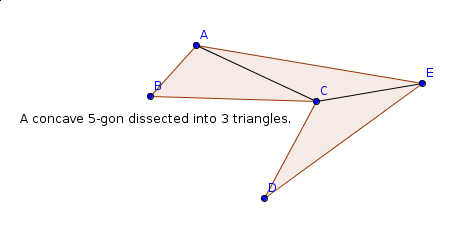
\includegraphics[scale=.5]{44-1}
            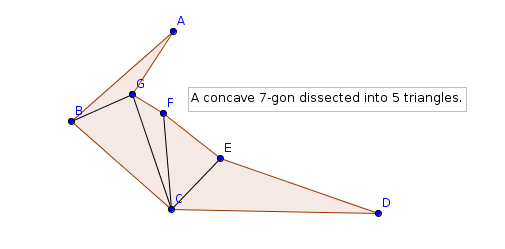
\includegraphics[scale=.5]{44-2}
        \end{center}
    \end{solution}
\end{exercise}

\begin{exercise}{45}
    Prove that every lattice triangle can be dissected into primitive lattice triangles.
    \begin{solution}
        This solution is probably the best I can do for this problem without neglecting the other (more interesting) problems from this check. I still think it's pretty good, but some things could probably be tightened up, like the set definitions for the points, and perhaps limiting the induction in some way.

        We will partition this problem into two smaller ones. We will first show that any lattice triangle can be dissected into lattice triangles whose only lattice boundary points are its vertices, and we will then show that any lattice triangle can be dissected into lattice triangles with no interior lattice points.

        Let \( n = 1. \) Suppose we have a lattice triangle with one non-vertex boundary lattice point, \( D. \) Simply connect \( D \) to its opposite vertex, and we have dissected the triangle into lattice triangles with no non-vertex boundary points.
        \begin{center}
            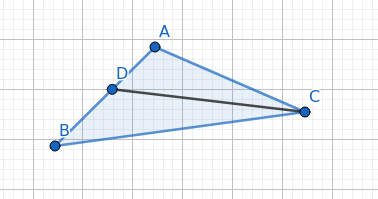
\includegraphics[scale=.5]{45-1}
        \end{center}
        For the purpose of induction, assume that for \( 1 \leq l < n , \) a lattice triangle with \( l \) non-vertex lattice boundary points can be dissected into lattice triangles with no non-vertex lattice boundary points. Let \( i,j,k \in \Z^{+} \cup \{0\} \) such that \( i \) is the number of non-vertex boundary lattice points on \( AB, \) \( j \) the same for \( BC, \) and \( k \) the same for \( AC. \) Let
        \begin{align*}
            \mathcal{A} &= \{P_{i'} : i' \leq  i \text{ and } P_{i'} \text{ is a non-vertex lattice boundary point on AB } \}\\
            \mathcal{B} &= \{R_{j'} : j' \leq  j \text{ and } R_{j'} \text{ is a non-vertex lattice boundary point on BC } \}\\
            \mathcal{C} &= \{Q_{k'} : k' \leq  k \text{ and } Q_{k'} \text{ is a non-vertex lattice boundary point on AC } \}\\
        \end{align*}
        \begin{center}
            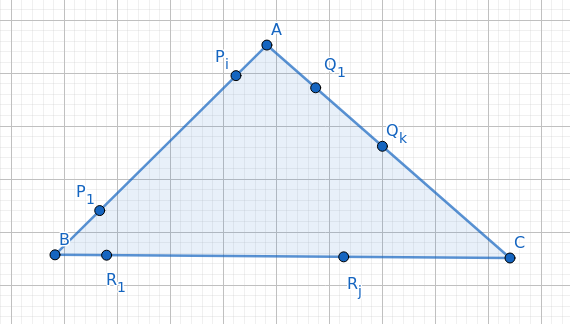
\includegraphics[scale=.5]{45-2}
        \end{center}
        For all \( i' \leq i, \) draw the segment \( P_{i'} C. \) For all \( j' \leq j ,\) draw the segment \( P_{1} R_{j'} . \) For all \( k' \leq k , \), draw the segment \( P_{n} Q_{k'} . \)
        \begin{center}
            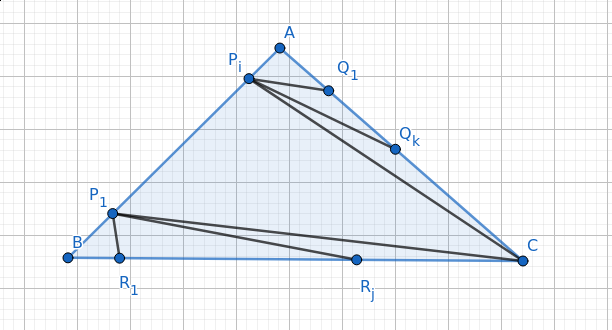
\includegraphics[scale=.5]{45-3}
        \end{center}
        We have created a series of lattice triangles, all of whom have strictly less than \( n \) non-vertex lattice boundary points. By the inductive hypothesis, we conclude that each of these triangles can be dissected into lattice triangles with no non-vertex lattice boundary points. These triangles partition our original triangle, so the original has the same property.

        Now we will show that every lattice triangle can be dissected into lattice triangles which have no interior lattice points. We will do so by induction on the number of interior lattice points.

        Let \( n = 1 \) and suppose a lattice triangle has \( n \) interior lattice points. Simply connect the segments between this interior point and the vertices of the triangle. Since the connected point is the only interior lattice point, the three created triangles have no interior lattice points. Thus the original can be dissected into lattice triangles with no interior lattice triangles.
        \begin{center}
            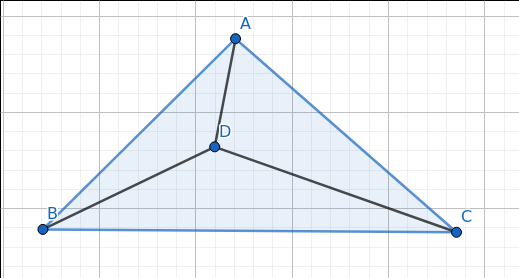
\includegraphics[scale=.5]{45-4}
        \end{center}
        Suppose that for \( 1 \leq l \leq n, \) if a lattice triangle has \( l \) interior lattice points, that triangle can be dissected into triangles with no interior lattice points. Choose an interior point \( D, \) and, as above, connect \( D \) to each vertex of the lattice triangle. We have created three lattice triangles, each of which have a strictly less number of interior lattice points than the original triangle, because \( D \) cannot be an interior lattice point for any of the triangles. By induction, each of these triangles may be dissected in the required way, and therefore the original can as well.

        We combine these two results to give the required result. Given a lattice triangle, that triangle can be dissected into lattice triangles which contain no non-vertex boundary points. Moreover, those triangles can be dissected into lattice triangles which contain no interior lattice points. The result is a lattice triangle which has been dissected into primitive lattice triangles.
    \end{solution}
\end{exercise}

\begin{exercise}{46}
    Prove that every lattice polygon can be dissected into primitive lattice triangles.
    \begin{solution}
        Let \( P \) be a lattice polygon. Since each vertex is a lattice point, the triangles which partition the polygon from exercise 44 are guaranteed to be lattice points. These are lattice triangles, and by 45, they can be dissected into primitive lattice triangles. Thus \( P \) can be dissected into primitive lattice triangles.
    \end{solution}
\end{exercise}
\pagebreak

\begin{exercise}{47}
    Dissect the twelve lattice polygons in Figure 3 into primitive lattice triangles. Note: you do not need to reproduce these drawings when you turn in your portfolio, but you will need the dissections when you complete Exercise 57.
    \begin{solution}
        See the picture below.
        \begin{center}
            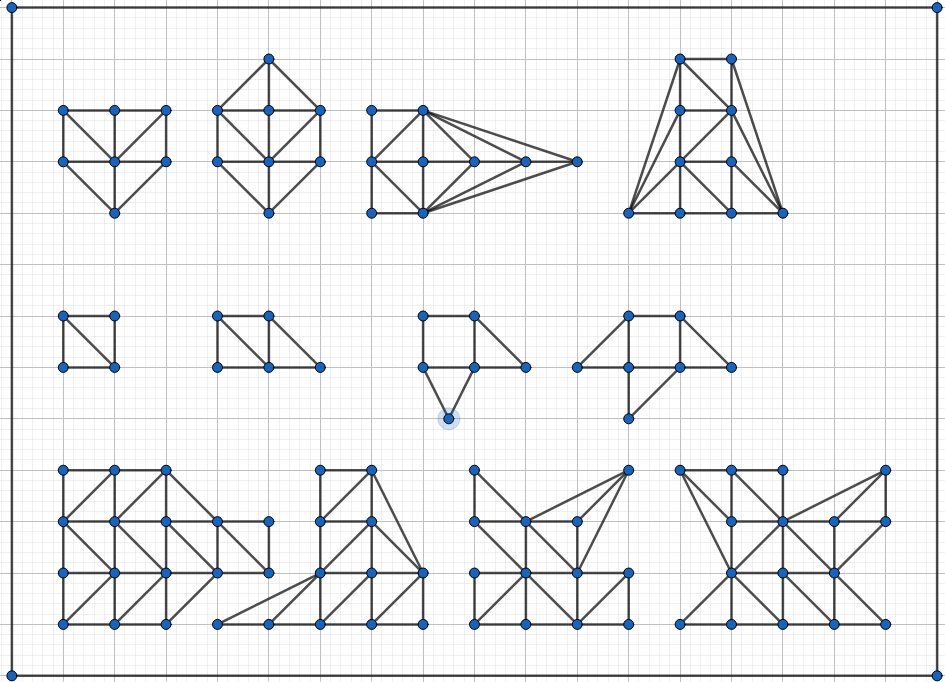
\includegraphics[scale=.5]{47}
        \end{center}
    \end{solution}
\end{exercise}

\begin{exercise}{48}
    Use Definition 22 to show that the two drawings below actually represent the same graph.
    \begin{center}
        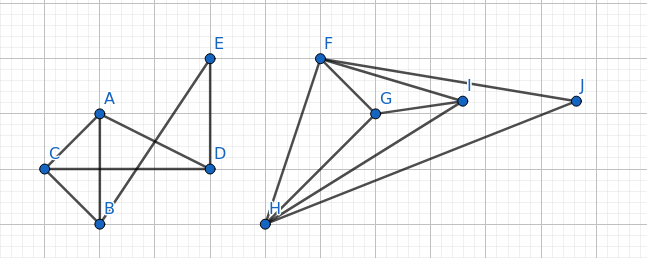
\includegraphics[width=.5\linewidth]{48}
    \end{center}
    \begin{solution}
        Definition 22 says that a graph is a tuple \( G = (V, E) \) consisting of a nonempty, finite set \( V \) of vertices and a finite set \( E \) of unordered pairs of distinct elements of \( V \) called edges. Let \( G_{1} = (V_{1} , E_{1}) \) be the left graph, and \( G_{2} = V_{2} , E_{2} \) be the right graph. Then \( V_{1} = \{1, 2, 3, 4, 5\} \) and \( V_{2} = \{1,2,3,4,5\} . \) These sets are equal, since they are clearly subsets of each other. Moreover, \( E_{1} = \{\{1,2\} , \{1, 3\} , \{1,4\}, \{2, 4\}, \{2,3\} , \{3,4\} , \{3, 5\} , \{4,5\} \} . \) \( E_{2} \) consists of exactly the same unordered pairs of vertices, so the two sets are the same. Thus \( G_{1} = (V_{1} , E_{1}) = (V_{2} , E_{2}) = G_{2} . \)
    \end{solution}
\end{exercise}

\begin{exercise}{49}
    Show that the graph shown below is a planar graph.
    \begin{center}
        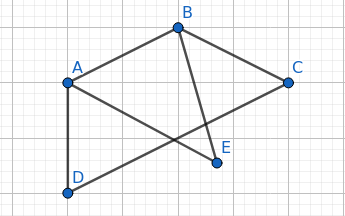
\includegraphics[width=.5\linewidth]{49-1}
    \end{center}
    \begin{solution}
        Below is the same graph drawn so that no two edges cross. Since this is demonstrably possible, the graph is planar.
    \begin{center}
        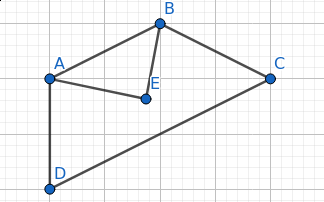
\includegraphics[width=.5\linewidth]{49-2}
    \end{center}
    \end{solution}
\end{exercise}\pagebreak
\begin{exercise}{50}
    Show that the graph illustrated below contains a circuit.
    \begin{center}
        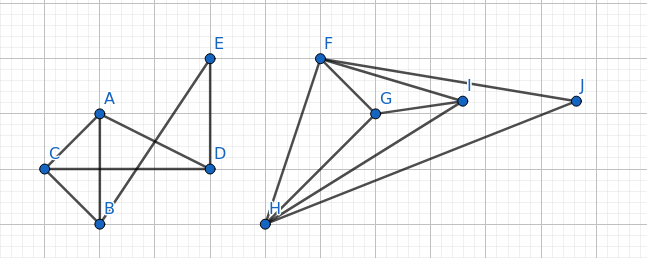
\includegraphics[width=.5\linewidth]{48}
    \end{center}
    \begin{solution}
        Consider the path \( \{1,2,4,1\} . \) This is a path since no edges repeat and the only vertices which repeat are the first and last. Since no other vertices repeat, the path is a circuit.
    \end{solution}
\end{exercise}

\begin{exercise}{51}
    Prove that if \( G \) is a tree, then there is a unique path between any two vertices of \( G. \)
    \begin{solution}
        Let \( G \) be a tree. Let \( v_{1} \) and \( v_{2} \) be a pair of distinct vertices of \( G. \) Since \( G \) is a tree, \( G \) is connected, and thus there is a path between \( v_{1} \) and \( v_{2} . \) We will now show the path is unique.

        Suppose for the sake of contradiction that there exist two distinct paths from \( v_{1} \) to \( v_{2}  \),
        \begin{align*}
            A &= \{v_{i_{1}} , \dots , v_{i_{n}}\} \\
            B &= \{v_{k_{1}} , \dots , v_{k_{m}}\}
        \end{align*}
        where \( v_{i_{1}} = v_{k_{1}} = v_{1} \) and \( v_{i_{n}} = v_{k_{m}} = v_{2} . \) Since the paths are distinct, there exists a \(1 \leq  t \leq \min(n,m)\) such that \( v_{i_{t}} \neq v_{k_{t}}  .\) Choose the smallest such \( t. \) Also, since \( v_{i_{n}} = v_{k_{m}} , \) there exists a \( 1 \leq s \leq \min(n,m) \) such that \( v_{i_{s}} = v_{k_{s}} . \) Choose the smallest such \( s \) which is greater than or equal to \( t. \) It is possible to make such a choice since the two paths must converge after their first divergence. Now \(t \leq s \leq \min(n,m) \). Consider the path
        \begin{align*}
            C = \{v_{i_{t-1}} , v_{i_{t}} , \dots , v_{i_{s}} = v_{k_{s}} , v_{k_{s-1}} , \dots , v_{k_{t-1}} = v_{i_{t-1}}\} .
        \end{align*}
        There cannot be any duplicate vertices other than \( v_{i_{t-1}} \) and \( v_{k_{t-1}} \) in the path since \( s \) was chosen as the smallest index such that \( v_{i_{s}} = v_{k_{s}} . \) Thus \( C \) is a cycle, but \( G \) is a tree and cannot contain cycles. We have a contradiction.

    \end{solution}
\end{exercise}

\begin{exercise}{52}
    Let \( v \) denote the number of vertices and let \( e \) denote the number of edges of \( G. \) Prove that if \( G \) is a tree, then \( e = v-1. \)
    \begin{solution}
        Fix a vertex \( u \) in \( G. \) Let \( A \) be the set of distinct paths from \( u \) to \( w_{i} \) for \( 1 \leq i \leq v \), or
        \begin{align*}
            A = \{\{u, \dots , w_{i}\} : 1 \leq i \leq v\} .
        \end{align*}
        Since \( G \) is a tree, there is a unique path between \( u \) and each of the other \( v-1 \) vertices of \( G. \) Thus \( \left| A \right| = v-1. \) We will show \( e = v-1 \) by proving \( \left| A \right| = \left| E \right| . \)

        Let \( \varphi : A \to E \) be the function which gives the last edge along the given path in \( A. \) The map is clearly well-defined, since the last edge of a unique path must be unique. We will begin by showing the map is onto. Let \( e \) be an arbitrary edge in \( E. \) Then there exist \( v_{1} , v_{2} \in V \) such that \( e = \{v_{1} , v_{2}\} . \) There are two cases:
        \begin{enumerate}
            \item Suppose one of \( v_{1} \) or \( v_{2} \) is \( u. \) Assume without loss of generality that \( v_{1} = u, \) so \( e = \{u, v_{2}\} . \) Here, the unique path from \( u \) to \( v_{2} \) is the path \( \{u, v_{2}\} , \) or simply the edge \( e. \) Thus \( \varphi(\{u, v_{2}\}) = e \) since \( e \) is the last and only edge of \( \{u , v_{2}\} . \)
            \item Assume neither \( v_{1} \) nor \( v_{2} \) are \( u. \) Since \( G \) is a tree, there is a unique path from \( u \) to \( v_{1} , \) namely \( \{u, \dots , v_{1} \}.  \) If \( e \) is the last edge of said path, \( \varphi(\{u , \dots , v_{1}\} ) = e \). If \( e \) is not the last edge, then \( \{u, \dots , v_{1} , v_{2}\} \) is the unique path from \( u \) to \( v_{2} , \) and the last edge of this path is \( e. \) Thus \( \varphi(\{u, \dots , v_{2}\}) = e. \)
        \end{enumerate}
        We will now show the map is 1-1. Suppose for the purpose of contradiction that \( \varphi \) is not 1-1, i.e. that there exist distinct paths \( \{u , \dots , w_{i}\} \) and \( \{u , \dots , w_{j}\} \) who share a last edge. Since the paths are distinct, \( w_{i} \neq w_{j} , \) since trees have unique paths. Also, since the paths share a last edge, we know \( \{u, \dots , w_{i}\} = \{u, \dots , w_{j} , w_{i}\} \) by definition of edge. Moreover, \( \{u, \dots , w_{j}\} = \{u, \dots , w_{i} , w_{j}\} . \) Thus, \( \{u , \dots, w_{i}\} = \{u , \dots , w_{i} , w_{j} , w_{i} \} . \) Thus a path in a tree contains a cycle \( \{w_{i} , w_{j} , w_{i}\} , \) which is impossible. We have a contradiction, and \( \varphi \) is 1-1.
    \end{solution}
\end{exercise}

\begin{exercise}{53}
    For each of the graphs below, find the number of vertices \( v, \) edges \( e, \) and regions \( f. \) Then compute \( v-e+f. \)
    \begin{center}
        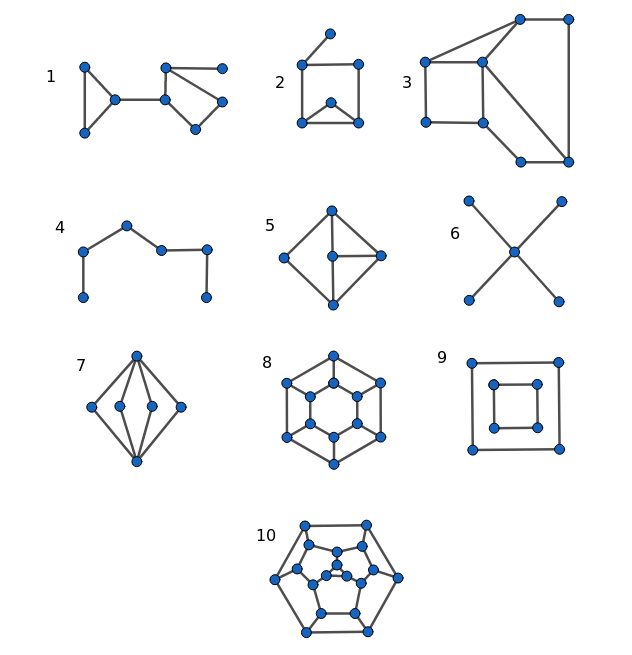
\includegraphics[scale=.5]{53}
    \end{center}
    \begin{solution}
        Below is the chart.
        \begin{center}
            \begin{tabular}{| c | c | c | c | c |}
                \hline
                Graphs & Vertices & Edges & Regions & \( v-e+f \)\\
                \hline
                \hline
                1 & 8 & 9 & 3 & 2\\
                2 & 6 & 7 & 3 & 2\\
                3 & 8 & 11 & 5 & 2\\
                4 & 6 & 5 & 1 & 2\\
                5 & 5 & 7 & 4 & 2\\
                6 & 5 & 4 & 1 & 2\\
                7 & 6 & 8 & 4 & 2\\
                8 & 12 & 18 & 8 & 2\\
                9 & 8 & 12 & 6 & 2\\
                10 & 18 & 27 & 11 & 2\\
                \hline
            \end{tabular}
        \end{center}
    \end{solution}
\end{exercise}

\begin{theorem}{7 Euler's Formula}
    If \( G \) is a connected, planar graph with \( v \) vertices, \( e \) edges, and \( f \) regions, then:
    \begin{align*}
        v-e+f = 2.
    \end{align*}
\end{theorem}

\begin{exercise}{54}
    Show that Euler's formula holds for the base case \( e = 0. \)
    \begin{solution}
        Suppose \( e = 0. \) There are 0 edges in \( G \) and \( G \) is a connected graph, so \( G \) must have one vertex only. Moreover, \( G \) does not divide the plane into any regions, so \( f = 1. \) Thus \( v + f = 2. \)
    \end{solution}
\end{exercise}

\begin{exercise}{55}
    \textit{Case 1:} Suppose that \( G \) does not contain a circuit. Then \( G \) is a tree. Use Exercise 52 to show that \( v-e+f = 2 \) in this case.
    \begin{solution}
        Suppose \( G \) does not contain a circuit, i.e. \( G \) a tree. Then \( e = v-1 \). So \( v - e + f = v - v + 1 + f = f + 1. \) Now a tree does not divide the plane into any additional regions, so \( f = 1 . \) Thus \( v -e + f = f + 1 = 2. \)
    \end{solution}
\end{exercise}

\begin{exercise}{56}
    \textit{Case 2:} Suppose that \( G \) contains a circuit \( C. \) In this case, \( e \geq 3. \) Now, let \( g \) be any edge of the circuit \( C, \) and consider the subgraph \( G' \) that consists of \( G \) with the edge \( g \) removed.
    \begin{enumerate}[label=(\alph*)]
        \item How many regions does \( G' \) have?
        \item How many vertices does \( G' \) have?
        \item How many edges does \( G' \) have?
        \item Use the inductive hypothesis to show that \( v-e+f=2. \)
    \end{enumerate}
    \begin{solution}
        \begin{enumerate}[label=(\alph*)]
            \item \( G' \) has \( f-1 \) regions, since we have removed an edge which is part of a circuit, and we have thus removed the face created by that circuit.
            \item We have removed no edges, so \( G' \) has \( v \) vertices.
            \item We've removed one edge, so \( G' \) has \( e-1 \) edges.
            \item \( G' \) is a connected planar graph with \( e-1 \) edges, so the inductive hypothesis yields
                \begin{align*}
                    v - (e-1) + (f-1) &= 2\\
                    v - e + 1 + f - 1 &= 2\\
                    v - e + f &= 2.
                \end{align*}
                Thus \( v-e+f = 2. \)
        \end{enumerate}
    \end{solution}
\end{exercise}

\begin{exercise}{57}
    By Theorem 5, we know that \( P \) has a dissection into primitive lattice triangles. Observe that since the sides of the triangles in the dissection of \( P \) do not intersect, and since the triangles are primitive, each lattice point in \( P \) is a vertex of a triangle. This dissection makes \( P \) a connected planar graph \( G \) as follows. The vertices of the graph \( G \) are the lattice points in \( P \) and on the sides of \( P. \) The edges of the graph \( G \) are the sedes of the primitive lattice triangles that triangulate \( P. \) Demonstrate this construction by using the polygons shown in Figure 3. For each of the polygons in Figure 3, use your dissection into primitive lattice triangles from Exercise 47 to construct the graph \( G. \) Let \( e_{i} \) denote the number of edges of \( G \) \textit{inside} the polygon \( P \) and let \( e_{b} \) denote the number of edges of \( G \) that are on the \textit{boundary}of the original polygon \( P. \) Finally, compute the quantity \( 2v-e_{b} -1. \) Complete the following table. What do you observe?
    \begin{solution}
        The picture below contains our dissections from 47.
        \begin{center}
            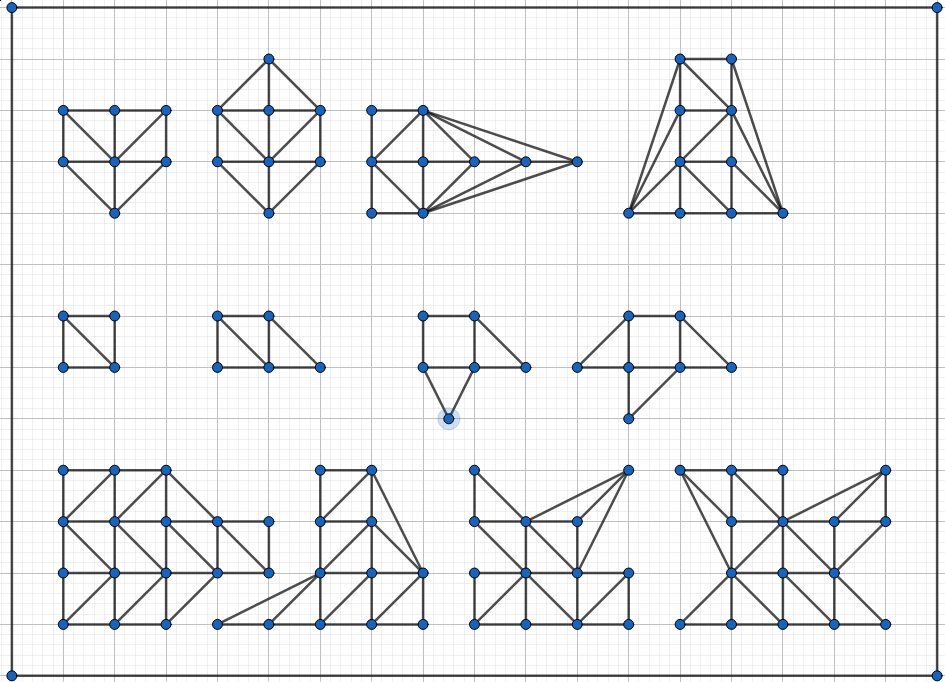
\includegraphics[scale=.4]{47}
        \end{center}
        The table below as requested.
        \begin{center}
            \begin{tabular}{| c | c | c | c |}
                \hline
                Polygon & Area of \( P \) & \( f = \# \) of regions of \( G \) & \( 2v-e_{b} -1 \) \\
                \hline
                \hline
                1 & 3 & 7 & 7\\
                2 & 4 & 9 & 9\\
                3 & 5 & 11 & 11\\
                4 & 6 & 13 & 13\\
                5 & 1 & 3 & 3\\
                6 & 1.5 & 4 & 4\\
                7 & 2 & 5 & 5\\
                8 & 2.5 & 6 & 6\\
                9 & 9 & 19 & 19\\
                10 & 6 & 13 & 13\\
                11 & 6 & 13 & 13\\
                12 & 8.5 & 18 & 18\\
                \hline
            \end{tabular}
        \end{center}
        Well, would you look at that? It would seem that the number of regions of these special \( G \) graphs are exactly \( 2v-e_{b} -1. \)
    \end{solution}
\end{exercise}

\begin{exercise}{58}
    Use Exercise 43 to state and prove an equation that relates the area of \( P \) to \( f . \)
    \begin{solution}
        We claim
        \begin{align*}
            A(P) = \frac{f-1}{2} .
        \end{align*}
        By exercise 43, the area of a primitive triangle is \( \frac{1}{2} . \) Each region of our graph other than the unbounded region is a lattice triangle. Thus we have \( (f-1) \) primitive triangles, whose areas we can add to give us the area of \( P. \) Thus \( A(P) = \frac{1}{2} (f-1) = \frac{f-1}{2} . \)
    \end{solution}
\end{exercise}

\begin{exercise}{59}
    The next step in the proof of Pick's Theorem is to compute \( e \) and relate it to \( f. \) Let \( e_{i} \) denote the number of edges of \( G \) \textit{inside} the polygon \( P \) and let \( e_{b} \) denote the number of edges of \( G \) that are on the \textit{boundary} of the original polygon \( P. \) Show that
    \begin{align*}
        f = 2v - e_{b} -1.
    \end{align*}
    \begin{solution}
        Note that \( e = e_{i} + e_{b} . \) Also, our graph consists of \( P \) dissected into \( f-1 \) primitive triangles. We will count the number of primitive lattice triangle sides present in our graph in two ways. First, each of the $f-1$ triangles have three sides. Also, each edge counted by $e_b$ is a side of one triangle, and each edge counted by $e_i$ is a side of two triangles. Counting the total number of sides,
        \begin{align*}
            3(f-1) = 3f - 3 &= e_{b} + 2 e_{i} \\
            &= e_{b} + 2 (e - e_{b}) \\
            &= e_{b} + 2e - 2 e_{b} \\
            &= 2e - e_{b} .
        \end{align*}
        Thus \( e = \frac{3}{2} f + \frac{1}{2} e_{b} - \frac{3}{2}. \) By Euler's theorem, \( e = v-2+f . \) Substituting,
        \begin{align*}
            v-2+f &= \frac{3}{2} f + \frac{1}{2} e_{b} - \frac{3}{2} \\
            -\frac{1}{2} f &= \frac{1}{2} e_{b} - \frac{3}{2} -v +2\\
            f &= -e_{b} + 3 + 2v - 4\\
            f &= 2v - e_{b} -1
        \end{align*}
    \end{solution}
\end{exercise}

\begin{exercise}{60}
    Finally, show that
    \begin{align*}
        A(P) = \frac{1}{2} B(P) + I(P) -1 .
    \end{align*}
    \begin{solution}
        Let \( P \) be an arbitrary lattice \( n \)-gon. By exercise 58, we have
        \begin{align*}
            A(P) = \frac{f-1}{2} .
        \end{align*}
        We know \( f = 2v- e_{b} - 1 \) by exercise 59, so
        \begin{align*}
            A(P) = \frac{2v-e_{b} -2}{2} = v - \frac{1}{2} e_{b} - 1 .
        \end{align*}
        For each boundary edge, there are two boundary points. Let
        $$ E_{b} = \{e_{j} : 1 \leq j \leq e_{b} \text{ and } e_{j} \text{ is a boundary edge of } P\} . $$
        Then by the inclusion-exclusion principle,
        \begin{align*}
            B(P) &= \sum_{e_{j} \in E_{b}} \left| e_{j} \right|\  - \sum_{1 \leq j \neq k \leq e_{b}} \left| e_{j} \cap e_{k} \right|\\
            &= 2 e_{b} \ - \sum_{1 \leq j \leq e_{b} -1} \left|e_{j} \cap e_{j+1}\right|\\
            &= 2 e_{b}\  - B(P)\\
            \implies B(P) &= e_{b} .
        \end{align*}
        Also, \( v = B(P) + I(P) \) since each point counted by \( B(P) \) and \( I(P) \) is a vertex of \( G. \) Thus
        \begin{align*}
            A(P) &= v - \frac{1}{2} e_{b} - 1 \\
            &= B(P) + I(P) - \frac{1}{2} B(P) -1\\
            &= \frac{1}{2} B(P) + I(P) -1.
        \end{align*}
    \end{solution}
\end{exercise}
\end{document}
